\documentclass[11pt,compress,t,notes=noshow, xcolor=table]{beamer}
\usepackage[]{graphicx}\usepackage[]{color}
% maxwidth is the original width if it is less than linewidth
% otherwise use linewidth (to make sure the graphics do not exceed the margin)
\makeatletter
\def\maxwidth{ %
  \ifdim\Gin@nat@width>\linewidth
    \linewidth
  \else
    \Gin@nat@width
  \fi 
}
\makeatother

\definecolor{fgcolor}{rgb}{0.345, 0.345, 0.345}
\newcommand{\hlnum}[1]{\textcolor[rgb]{0.686,0.059,0.569}{#1}}%
\newcommand{\hlstr}[1]{\textcolor[rgb]{0.192,0.494,0.8}{#1}}%
\newcommand{\hlcom}[1]{\textcolor[rgb]{0.678,0.584,0.686}{\textit{#1}}}%
\newcommand{\hlopt}[1]{\textcolor[rgb]{0,0,0}{#1}}%
\newcommand{\hlstd}[1]{\textcolor[rgb]{0.345,0.345,0.345}{#1}}%
\newcommand{\hlkwa}[1]{\textcolor[rgb]{0.161,0.373,0.58}{\textbf{#1}}}%
\newcommand{\hlkwb}[1]{\textcolor[rgb]{0.69,0.353,0.396}{#1}}%
\newcommand{\hlkwc}[1]{\textcolor[rgb]{0.333,0.667,0.333}{#1}}%
\newcommand{\hlkwd}[1]{\textcolor[rgb]{0.737,0.353,0.396}{\textbf{#1}}}%
\let\hlipl\hlkwb

\usepackage{framed}
\makeatletter
\newenvironment{kframe}{%
 \def\at@end@of@kframe{}%
 \ifinner\ifhmode%
  \def\at@end@of@kframe{\end{minipage}}%
  \begin{minipage}{\columnwidth}%
 \fi\fi%
 \def\FrameCommand##1{\hskip\@totalleftmargin \hskip-\fboxsep
 \colorbox{shadecolor}{##1}\hskip-\fboxsep
     % There is no \\@totalrightmargin, so:
     \hskip-\linewidth \hskip-\@totalleftmargin \hskip\columnwidth}%
 \MakeFramed {\advance\hsize-\width
   \@totalleftmargin\z@ \linewidth\hsize
   \@setminipage}}%
 {\par\unskip\endMakeFramed%
 \at@end@of@kframe}
\makeatother

\definecolor{shadecolor}{rgb}{.97, .97, .97}
\definecolor{messagecolor}{rgb}{0, 0, 0}
\definecolor{warningcolor}{rgb}{1, 0, 1}
\definecolor{errorcolor}{rgb}{1, 0, 0}
\newenvironment{knitrout}{}{} % an empty environment to be redefined in TeX

\usepackage{alltt}
\newcommand{\SweaveOpts}[1]{}  % do not interfere with LaTeX
\newcommand{\SweaveInput}[1]{} % because they are not real TeX commands
\newcommand{\Sexpr}[1]{}       % will only be parsed by R

\usepackage[english]{babel}
\usepackage[utf8]{inputenc}
\usepackage{dsfont}
\usepackage{verbatim}
\usepackage{amsmath}
\usepackage{amsfonts}
\usepackage{bm}
\usepackage{csquotes}
\usepackage{multirow}
\usepackage{longtable}
\usepackage{booktabs}
\usepackage{enumerate}
\usepackage[absolute,overlay]{textpos}
\usepackage{psfrag}
\usepackage{algorithm}
\usepackage{algpseudocode}
\usepackage{eqnarray}
\usepackage{arydshln}
\usepackage{tabularx}
\usepackage{placeins}
\usepackage{tikz}
\usepackage{setspace}
\usepackage{colortbl}
\usepackage{mathtools}
\usepackage{wrapfig}
\usepackage{bm}
\usepackage{xcolor}
\usetikzlibrary{shapes,arrows,automata,positioning,calc,chains,trees, shadows}
\tikzset{
  %Define standard arrow tip
  >=stealth',
  %Define style for boxes
  punkt/.style={
    rectangle,
    rounded corners,
    draw=black, very thick,
    text width=6.5em,
    minimum height=2em,
    text centered},
  % Define arrow style
  pil/.style={
    ->,
    thick,
    shorten <=2pt,
    shorten >=2pt,}
}
\usepackage{subfig}



% Defines macros and environments
\input{../../style/common.tex}

\usepackage{../../style/lmu-lecture}

\newcommand{\bfit}[1]{\textbf{\textit{#1}}}
\colorlet{highlightcol}{gray!80}
\newcommand{\maketag}[1]{\colorbox{highlightcol}{\textcolor{white}
{\MakeUppercase{#1}}}}
\newcommand{\highlight}[1]{\textcolor{highlightcol}{\textbf{#1}}}
\newcommand{\positem}{\item[$\highlight{+}$]}
\newcommand{\negitem}{\item[$\highlight{-}$]}
\newcommand{\conclbox}[1]{\fbox{\parbox{\textwidth}{\centering\textbf{#1}}}}

\let\code=\texttt
\let\proglang=\textsf

\setkeys{Gin}{width=0.9\textwidth}

\title{Models in Machine Learning}
\author{Bernd Bischl}
\institute{\href{https://compstat-lmu.github.io/lecture_i2ml/}
{compstat-lmu.github.io/lecture\_i2ml}}
\date{}

\setbeamertemplate{frametitle}{\expandafter\uppercase\expandafter
\insertframetitle}

\begin{document}

% Defines macros and environments
\input{../../latex-math/basic-math.tex}
\input{../../latex-math/basic-ml.tex}
\input{../../latex-math/ml-lm.tex}
\input{../../latex-math/ml-trees.tex}
\input{../../latex-math/ml-bagging.tex}
\input{../../latex-math/ml-boosting.tex}

%! includes: basics-learners

\lecturechapter{An Overview}
\lecture{Models in Machine Learning}

% ------------------------------------------------------------------------------
% LINEAR MODEL
% ------------------------------------------------------------------------------

\begin{frame}{Linear Model -- Functionality}

\footnotesize

\maketag{SUPERVISED}
\maketag{PARAMETRIC}
\maketag{WHITE-BOX}


\medskip


\highlight{General idea} ~~  
%\begin{itemize}
A linear model (LM) represents the target as a linear combination of the input variables.
%A linear model (LM) fits a \textbf{hyperplane} $\theta_0 + \thx$ to minimize the distance between the data points and its closed point on the hyperplane. 


%\item The linear model approximates the \textbf{linear influence} of the features on the target variable. 
%\item Thus, linear models can only perform \textbf{regression}, as they can only predict continuous, numeric values. 
%\end{itemize}

\medskip

\highlight{Hypothesis space} ~~
$\Hspace = \left\{f: \Xspace \to \R ~|~\fx = \phi(\thetab^\top \xv)\right\}$, 
where $\phi(\cdot): \R \to \Phi \subseteq \R$ is some transformation function.

\smallskip

For different $\phi(\cdot)$ it results in different models, e.g.: 
\begin{itemize}
  \item identity function $\phi(\thetab^\top \xv) = \thetab^\top \xv$ :  \textbf{linear regression} -- a \textbf{hyperplane} $\theta_0 + \thx$ is fitted to the data(regression task).
  \item logistic sigmoid function $\phi(\thetab^\top \xv) = \frac{1}{1 + \exp(- \thetab^\top \xv)} = \pix$ : \textbf{logistic regression} - the probability $\pix = \P(y = 1 ~|~\xv)$ is fitted by a \textcolor{blue}{wave} based on the logit link (inverse of logistic sigmoid function). Applying a decision rule (e.g., $\pix >0.5$) results in a separating hyperplane (classification task, linear classifier). 

\end{itemize}

%$\Hspace = \{ \theta_0 + \thx\ |\ (\theta_0, \thetab) \in \R^{p+1} \}$

% \textbf{Linear Model}: Used in different contexts, often a synonym for models in the class of linear pblueictors or for linear regression (with potentially transformed input space, i.e.,  $\yi = \thetab^\top \psi^{(i)}(\xi) + \varepsilon^{(i)}$, where $\psi^{(i)}(\cdot)$ can be non-linear functions transforming $\xi$). 

\footnotesize

\begin{minipage}{0.32\textwidth}
% from FCIM: lecture_cim2\2020\02-univariate-modelling\archive\slides-2-multi-linear.Rnw
  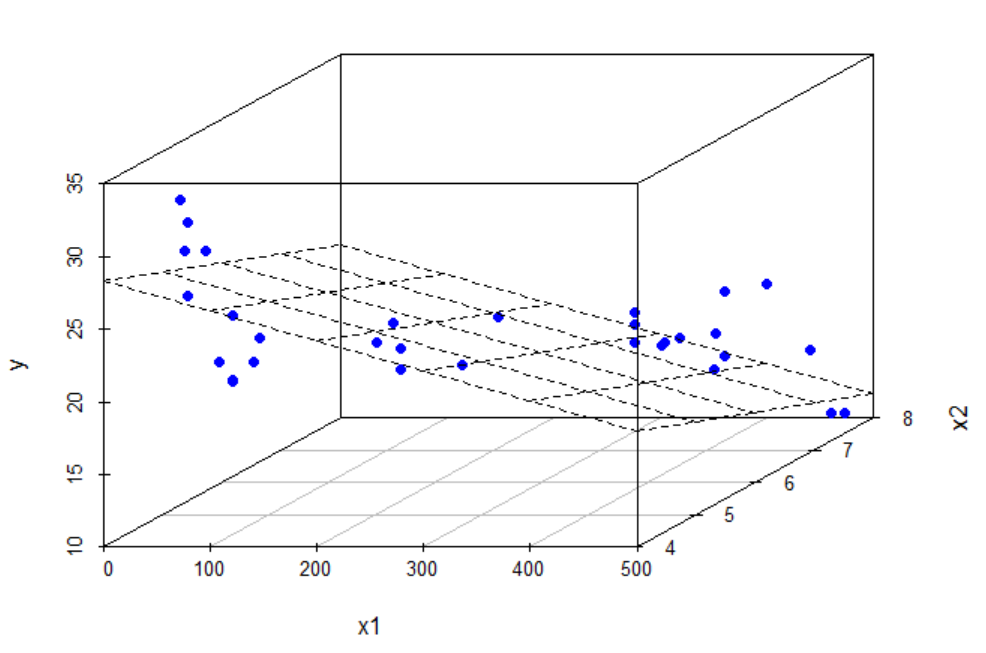
\includegraphics[width=1.05\textwidth]{figure/linreg-surface.png}
\end{minipage}
 \normalsize 
\begin{minipage}{0.42\textwidth}
  \begin{center}
% from FCIM: lecture_cim2\2020\02-univariate-modelling\figure_man
  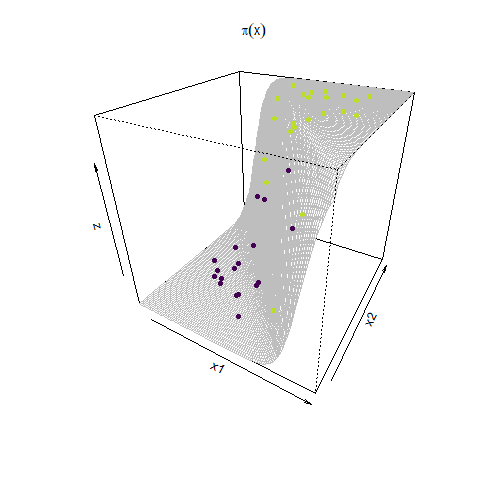
\includegraphics[width=0.75\textwidth]{figure/logreg-2vars-surface.png}
  \end{center}
\end{minipage}
\begin{minipage}{0.22\textwidth}
% from FCIM: lecture_cim2\2020\02-univariate-modelling\figure_man
  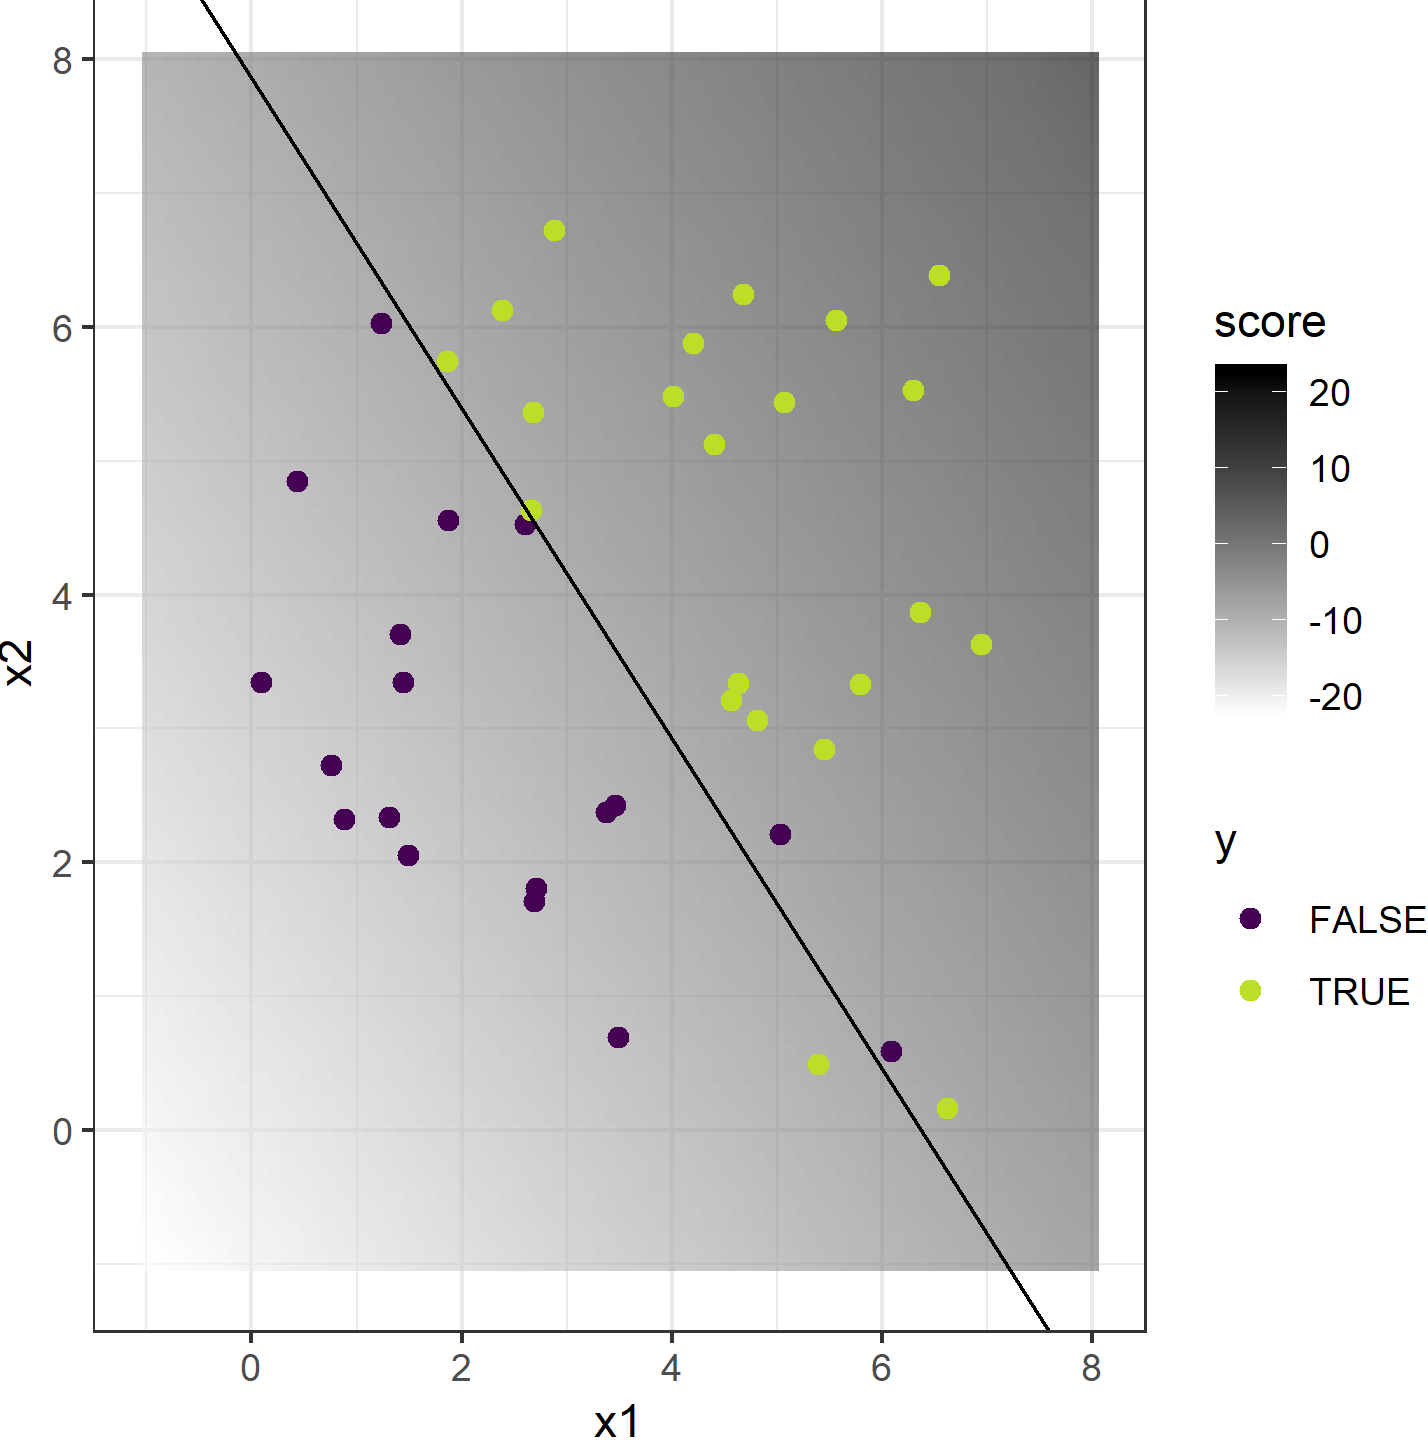
\includegraphics[width=\textwidth]{figure/logreg-2vars-data.png}
\end{minipage}

\end{frame}

% ------------------------------------------------------------------------------

\begin{frame}{Linear Model -- Functionality}

\footnotesize

\highlight{Empirical risk}
\begin{itemize}\footnotesize
  \item Typically, in \textbf{linear regression} the \textbf{ordinary least squares (OLS)} with a squared loss function is used for regression: $\risket  = \sumin \left(\yi - \thetab^T \xi\right)^2$
    
   \item Alternatively, the \textbf{absolute loss} or the \textbf{Huber loss} can be used. %$\risket = \sumin \left|\yi - \thetab^T \xi\right|$ 
  
  \item For \textbf{logistic regression} the risk function is based on the \textbf{Bernoulli loss} $\risket = \sumin -\yi \log \left(\pixii\right) - (1 - \yi) \log \left(1 - \pixii \right)$.
  
  %logistic loss \Lxy = \log \left[1 + \exp \left(-y\fx\right)\right].


\end{itemize}

\footnotesize

\medskip

\highlight{Optimization}
\begin{itemize}\footnotesize
  \item for \textbf{OLS}: analytically with $\bm{\hat \theta} = (\Xmat^\top \Xmat)^{-1} \Xmat^\top\ydat$
  ($\Xmat \in \R^{n \times p}$ : matrix of feature vectors)
  \item for \textbf{other loss functions}: numerical optimization 
\end{itemize}

\medskip

\highlight{Hyperparameters} ~~ None

\medskip

% \highlight{Runtime behavior} ~~ $\mathcal{O}(p^2 \cdot n + p^3)$ for $n$ 
% observations and $p$ features

\end{frame}

% ------------------------------------------------------------------------------

\begin{frame}{Linear Model -- Pro's \& Con's}

\footnotesize

\begin{columns}[onlytextwidth]
  \begin{column}{0.5\textwidth}
    \highlight{Advantages}
    \footnotesize
    \begin{itemize}
      \positem \textbf{simple and fast} implementation; cheap computational costs
      \positem intuitive \textbf{interpretability}: mean influence of features on the output and feature importance
      \positem fits \textbf{linearly} separable data sets very well
      \positem works well \textbf{independent of data size}
      \positem basis for many machine learning algorithms

    \end{itemize}
  \end{column}

  \begin{column}{0.5\textwidth}
    \highlight{Disadvantages}
    \footnotesize
    \begin{itemize}
      \negitem not suitable for data based on a \textbf{non-linear} data generating process $\rightarrow$ \textbf{strong simplification} of real-world problems
      
      \negitem \textcolor{blue}{\textbf{strong assumptions}: data is independent (multi-collinearity must be removed)}
      
      \negitem tend to \textbf{overfit} (can be reduced by regularization)
      
      \negitem \textbf{sensitive to outliers and noisy data}
    \end{itemize}
  \end{column}
\end{columns}

\vfill

\small

\conclbox{Simple method with good interpretability for linear problems, but strong assumptions and simplification of real-world problems}

\end{frame}

% ------------------------------------------------------------------------------

\begin{frame}{Linear Model -- Practical hints}

\footnotesize

 \highlight{\textcolor{blue}{Check assumptions??} }\\
 \textcolor{blue}{This model is very effective if the following assumptions are fulfilled:}
 \begin{itemize}\footnotesize
  \item \textbf{linearity}: The expected response is a linear combination of the features.
  \item \textbf{homoscedasticity}: The variance of residuals is equal for all features.
  \item \textbf{independence}: All observations are independent of each other.
  \item \textbf{normality}: Y is normally distributed for any fixed value of the features
\end{itemize}


\medskip

  \highlight{Implementation}
  
  \begin{itemize}
    \item \textbf{R:} \code{mlr3} learner \code{LearnerRegrLM}, calling \code{stats::lm()}
    \item \textbf{Python:} \code{LinearRegression} from package 
    \code{sklearn.linear\_model}, package for advanced statistical parameters 
    \code{statsmodels.api} 
  \end{itemize}

\medskip

 \highlight{Regularization} \\

 In practice, we often use regularized models in order to \textbf{prevent overfitting} or perform feature selection. More details will follow in the subsequent chapter. 


\end{frame}

% ------------------------------------------------------------------------------
% REGULARIZED LINEAR MODEL
% ------------------------------------------------------------------------------

\begin{frame}{Regularized LM -- Functionality}

\footnotesize

\maketag{SUPERVISED}
\maketag{PARAMETRIC}
\maketag{WHITE-BOX}

\medskip

\highlight{General idea} ~~
\begin{itemize}

\item Linear model (LM) can \textbf{overfit} if we operate in high-dimensional space with not that many observations.

\item When features are highly correlated, the OLS estimate becomes highly sensitive to random errors in the observed response, producing a \textbf{large variance in the fit}.

\item We can find a compromise between generalizing the model (simple model, underfitted) and corresponding closely to the data (complex model, overfitted).

\end{itemize}

\medskip

\highlight{Hypothesis space} ~~
$\Hspace = \left\{f: \Xspace \to \R ~|~\fx = \phi(\thetab^\top \xv)\right\}$, 
where $\phi(\cdot): \R \to \Phi \subseteq \R$ is some transformation function.


%$\Hspace = \{ \theta_0 + \thx\ |\ (\theta_0, \thetab) \in \R^{p+1} \} $

\medskip
% \footnotesize
% \begin{minipage}{0.5\textwidth}
\centering
  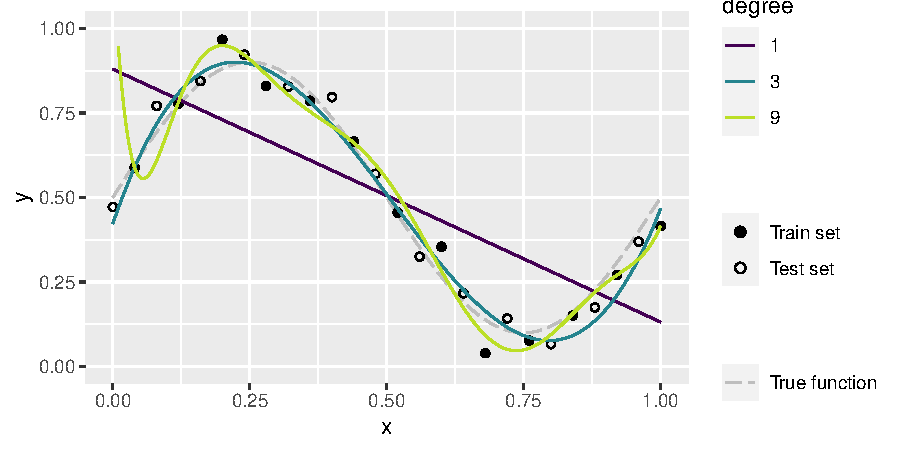
\includegraphics[width=0.6\textwidth]{figure/reg_lm_overfitting.pdf}
% \end{minipage}
%  \normalsize
% \begin{minipage}{0.4\textwidth}
%   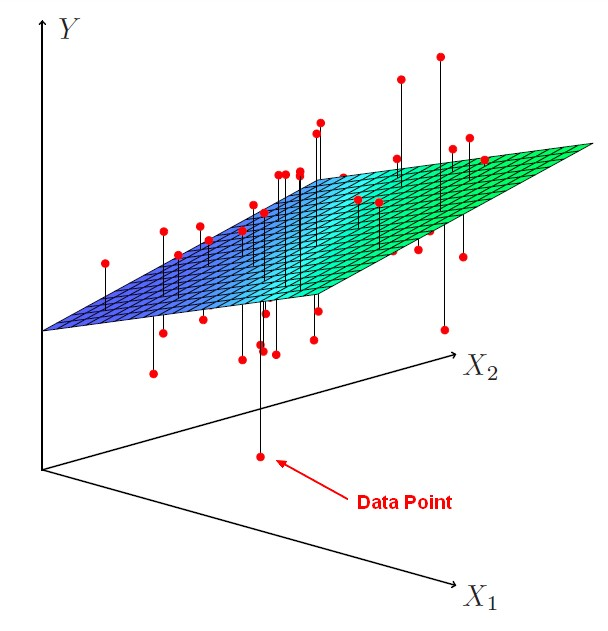
\includegraphics[width=0.7\textwidth]{figure/regression_hyperplane.jpg}
% \end{minipage}

\end{frame}

% ------------------------------------------------------------------------------

\begin{frame}{Regularized LM -- Functionality}

\footnotesize

\highlight{Empirical risk}

\begin{itemize}

\item Therefore, we minimize the empirical risk function $\risket$ \textbf{plus a complexity penalty} $J(\thetab)$, controlled by shrinkage parameter $\lambda$:
  $
  \riskrt = \risket + \lambda \cdot J(\thetab). 
  $ 
  
\item \textbf{Ridge regression} uses the L2-penalty as a complexity measure with $J(\thetab) = \|\thetab\|_2^2 $. 

\item Alternativly, \textbf{LASSO} (least absolute shrinkage and selection operator) uses the L1-penalty ($J(\thetab) = \|\thetab\|_1 $).

\item While both regularization methods shrink the coefficients of the model; LASSO also performs \textbf{feature selection}. 

\item \textbf{Elastic net} uses a convex combination of Ridge and LASSO with $J(\thetab) = \lambda_1 \|\thetab\|_1 + \lambda_2 \|\thetab\|_2^2$.
  
  
\end{itemize}





\medskip

\highlight{Optimization} ~~
\begin{itemize}\footnotesize
  \item for \textbf{Ridge} regression: analytically with $\thetah_{\text{Ridge}} = (\Xmat^T \Xmat  + \lambda \id)^{-1} \Xmat^T\ydat$
  \item for \textbf{LASSO regression}: e. g. (sub)-gradient descent
\end{itemize}

\medskip

\highlight{Hyperparameters} ~~ \textbf{Shrinkage parameter} $\lambda$ [or $\lambda_1$ and $\lambda_2$ for elastic net] \\

\medskip

% \highlight{Runtime behavior} ~~ $\mathcal{O}(p^2 \cdot n + p^3)$ for $n$ 
% observations and $p$ features 

\end{frame}

% ------------------------------------------------------------------------------

\begin{frame}{Regularized LM -- Pro's \& Con's}

\footnotesize

\textcolor{blue}{ALMOST SAME LIKE LINEAR MODEL?--> does this make sense?}

\begin{columns}[onlytextwidth]
  \begin{column}{0.5\textwidth}
    \highlight{Advantages}
    \footnotesize
    \begin{itemize}
      \positem simple and fast implementation; cheap computational costs
      \positem intuitive interpretability: mean influence of features on the output and feature importance
      \positem fits linearly separable data sets very well
      \positem works well independent of data size
      \positem basis for many machine learning algorithms
      \positem \textcolor{blue}{less tendency to \textbf{overfit}}

    \end{itemize}
  \end{column}

  \begin{column}{0.5\textwidth}
    \highlight{Disadvantages}
    \footnotesize
    \begin{itemize}
      \negitem not suitable for data based on a non-linear data generating process $\rightarrow$ strong simplification of real-world problems

      \negitem \textcolor{blue}{\textbf{strong assumptions}: data is independent (multi-collinearity must be removed and normal distributed residuals ??}

      \negitem sensitive to outliers and noisy data
    \end{itemize}
  \end{column}
\end{columns}

\vfill

\small

\conclbox{Simple method with good interpretability for linear problems, but strong assumptions and simplification of real-world problems.}

\end{frame}

% ------------------------------------------------------------------------------

\begin{frame}{Regularized LM -- Practical hints}

\footnotesize

  \highlight{Choice of regularization parameter  $\lambda$} \\

 Choose $\lambda$ with e. g. the smallest sum of squared residuals through cross-validation. \\
 In the R package \code{glmnet} \code{lambda.min} is the value of $\lambda$ that gives minimum mean cross-validated error.
 
\medskip

\highlight{Ridge vs. LASSO} \\
\begin{itemize}
    \item neither is overall better $\rightarrow$ elastic net as a compromise
    \item \textbf{Ridge} works better, if there are many influential and high correlated features. 
    \item In contrast, \textbf{LASSO} is more suitable if the underlying structure is sparse (only a few features influence the output $y$).
    \item LASSO can set coefficients to zero, thus performing \textbf{variable selection}. 
  \end{itemize}


\medskip

\highlight{Implementation}

\begin{itemize}
    \item \textbf{R:} \code{mlr3} learners \code{LearnerClassifGlmnet} / 
    \code{LearnerRegrGlmnet}, calling \code{glmnet::glmnet()}
    \item \textbf{Python:} \code{LinearRegression} from package 
    \code{sklearn.linear\_model}, package for advanced statistical parameters 
    \code{statsmodels.api} 
  \end{itemize}

\end{frame}

% ------------------------------------------------------------------------------
% Linear SVM
% ------------------------------------------------------------------------------

\begin{frame}{Linear SVM -- Functionality}

\footnotesize

\maketag{SUPERVISED}
\maketag{PARAMETRIC}
\maketag{BLACK-BOX}

\medskip

\highlight{General idea}
\begin{itemize}

%\item Support vector machines (SVMs) construct separating \textbf{hyperplanes} in a multi-dimenstional space.  

  \item The support vector machine (SVM) algorithm finds a decision boundary (\textbf{separating hyperplane}) that maximizes the distance (\textbf{margin $\gamma$}) to the closest members (\textbf{support vectors, SV}) of the separate classes. (\textbf{hard margin})
  
  %\item It is a \textbf{convex optimization problem} (quadratic program) which tries to maximize the \enquote{safety margin} where the distance of all data point to the hyperplane should be greater than the margin. 
  
  \item In a \textbf{soft-margin SVM} also \enquote{violations} of the margin are allowed $\rightarrow$ not only the margin should be maximized, but also the margin violations minimized. 
  
  %\item The parameter $C > 0$ controls this trade-off between the contradictonary goals. 
  
  \item There are three different types of training points: \textbf{Non-SVs} which do not influence the hyperplane, \textbf{SVs} which are exactly on the hyperplane, and \textbf{margin violators}. 
  
  
  
  


\end{itemize}

\medskip

% \operatorname{sign}(\mathbf{w} \cdot \Phi(\mathbf{x})+b)

\highlight{Hypothesis space} ~~
$\Hspace = \left\{f: \Xspace \to \R ~|~\fx = \thetab^\top \xv + \theta_0\right\}$

\medskip
 \footnotesize
 \begin{minipage}{0.6\textwidth}
    \centering
    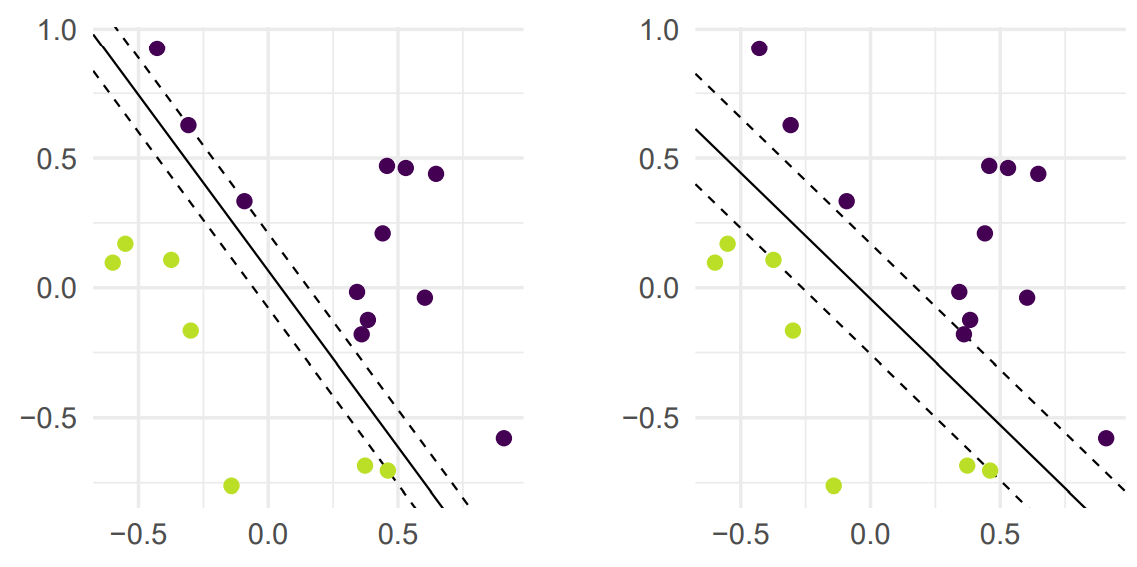
\includegraphics[width=0.9\textwidth]{figure/svm_motivation_hard_margin.png}
 \end{minipage}
  \normalsize
  \hfill\vline\hfill
 \begin{minipage}{0.3\textwidth}
    \centering
    %https://docs.google.com/presentation/d/1g7q1hbTNmQeuRWQIM8SF9l6iKWmJyuhyhm3s9QjA0jM/edit?usp=sharing
%from FCIM 2020/Linear SVM /slides-3-soft-margin (last plot, page8)
    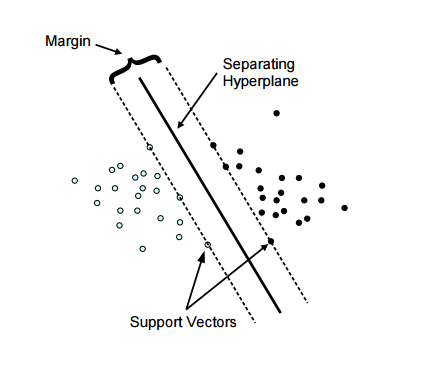
\includegraphics[width=1.1\textwidth]{figure/svm_wording.png}
 \end{minipage}

\end{frame}

% ------------------------------------------------------------------------------

\begin{frame}{Linear SVM -- Functionality}

\footnotesize

\highlight{Empirical risk}

Soft-margin SVMs can also be interpreted as \textbf{L2-regularized ERM}: 

$$ \frac{1}{2} \|\thetab\|^2 + C \sumin \Lxyi ;\; \Lyf = \max(1-yf, 0),$$ 
with $\Lyf$ as the hinge loss, $\|\thetab\| = 1 / \gamma$ and $C$ as cost parameter for margin violation.

\medskip

\highlight{Optimization} ~~
As the problem is \textbf{not differentiable}, there are the following solutions: 
\begin{enumerate}
\item Use a smoothed loss (squared hinge, huber), then do gradient descent.\\
  NB: Will not  create a sparse SVM if we do not add extra tricks.
\item Use \textbf{subgradient} methods.
\item Do stochastic subgradient descent.\\
  Pegasos: Primal Estimated sub-GrAdient SOlver for SVM.
\end{enumerate}

\medskip

\highlight{Hyperparameters} ~~ \textbf{$C$} : penalization for missclassified data points 


\medskip
%https://www.ijcaonline.org/research/volume128/number3/abdiansah-2015-ijca-906480.pdf
% \highlight{Runtime behavior} ~~ \textcolor{blue}{$\mathcal{O}(n^3)$ for $n$ observations} %$\mathcal{O}(n^2 \cdot p + n^3)$ for $n$ observations and $p$ features

\end{frame}

% ------------------------------------------------------------------------------

\begin{frame}{Linear SVM -- Pro's \& Con's}

\footnotesize


\begin{columns}[onlytextwidth]
  \begin{column}{0.5\textwidth}
    \highlight{Advantages}
    \footnotesize
    \begin{itemize}
      \positem high \textbf{accuaracy}
      \positem often \textbf{sparse} solution
      \positem robust against overfitting (\textbf{regularized}); especially in high-dimensional space
      \positem \textbf{stable} solutions, as the non-SV do not influence the separating hyperplane
      %\positem \textbf{memory efficient} (only use non-SVs)
    \end{itemize}
  \end{column}

  \begin{column}{0.5\textwidth}
    \highlight{Disadvantages}
    \footnotesize
    \begin{itemize}
      \negitem \textbf{costly implementation}; long training times
      \negitem does not scale well to \textbf{larger data sets} \textcolor{blue}{\textbf{??}}
      \negitem only \textbf{linear separation} $\rightarrow$ possible with non-linear SVMs which are explained in the following slides.
      \negitem poor \textbf{interpretability}
    \end{itemize}
  \end{column}
\end{columns}

\vfill

\small

\conclbox{Very accurate solution for high-dimensional data that is linearly separable}

\end{frame}

% ------------------------------------------------------------------------------

\begin{frame}{Linear SVM -- Practical hints}

\footnotesize

  \highlight{Preprocessing} \\
  Features must be rescaled before applying SVMs.
  
  \medskip
  
  \highlight{Tuning} \\
  The cost parameter $C$ must be tuned, as it has a strong influence on the resulting separating hyperplane. 

  \medskip

  \highlight{Implementation} 
  \begin{itemize}
    \item \textbf{R:} \code{mlr3} learners \code{LearnerClassifSVM} / 
    \code{LearnerRegrSVM}, calling \code{svm()} from \code{libsvm}
    \item \textbf{Python:} \code{sklearn.svm.SVC} from package \code{scikit-learn} / package \code{libSVM}
  \end{itemize}

\end{frame}

% ------------------------------------------------------------------------------
% Non-linear SVM
% ------------------------------------------------------------------------------

\begin{frame}{Non-linear SVM -- Functionality}

\footnotesize

\maketag{SUPERVISED}
\maketag{NON PARAMETRIC}
\maketag{BLACK-BOX}

\medskip

\highlight{General idea}
\begin{itemize}

  \item Non-linear SVMs construct a separating hyperplane in a \textbf{higher dimensional dimension}
  \item \textbf{Kernels = feature map + inner product} $k(\xv, \tilde \xv)$ transform the input space into a higher dimensional space and calculates the inner product. 

\end{itemize}

\medskip

% \operatorname{sign}(\mathbf{w} \cdot \Phi(\mathbf{x})+b)

\highlight{Hypothesis space} ~~
$\Hspace = \{ \fx = \sumin \alpha_i \yi k(\xi, \xv)  + \theta_0 |\ \theta_0, \alpha_i \in \R \} $
%\textcolor{blue}{$\Hspace = \{ \operatorname{sign}(\sumin \alpha_i \yi k(\xi, \xv)  + \theta_0) |\ (\theta_0, \thetab) \in \R^{p+1} \} $}

\medskip
 \footnotesize
 \begin{minipage}{0.48\textwidth}
\centering
  % from FCIM 2020 lecture_cim2\2020\09-nonlinear-svm\slides-1-featuregen.Rnw page 3
  $\phi(x_1, x_2) = (x_1, x_2, x_1^2+x_2^2)$
 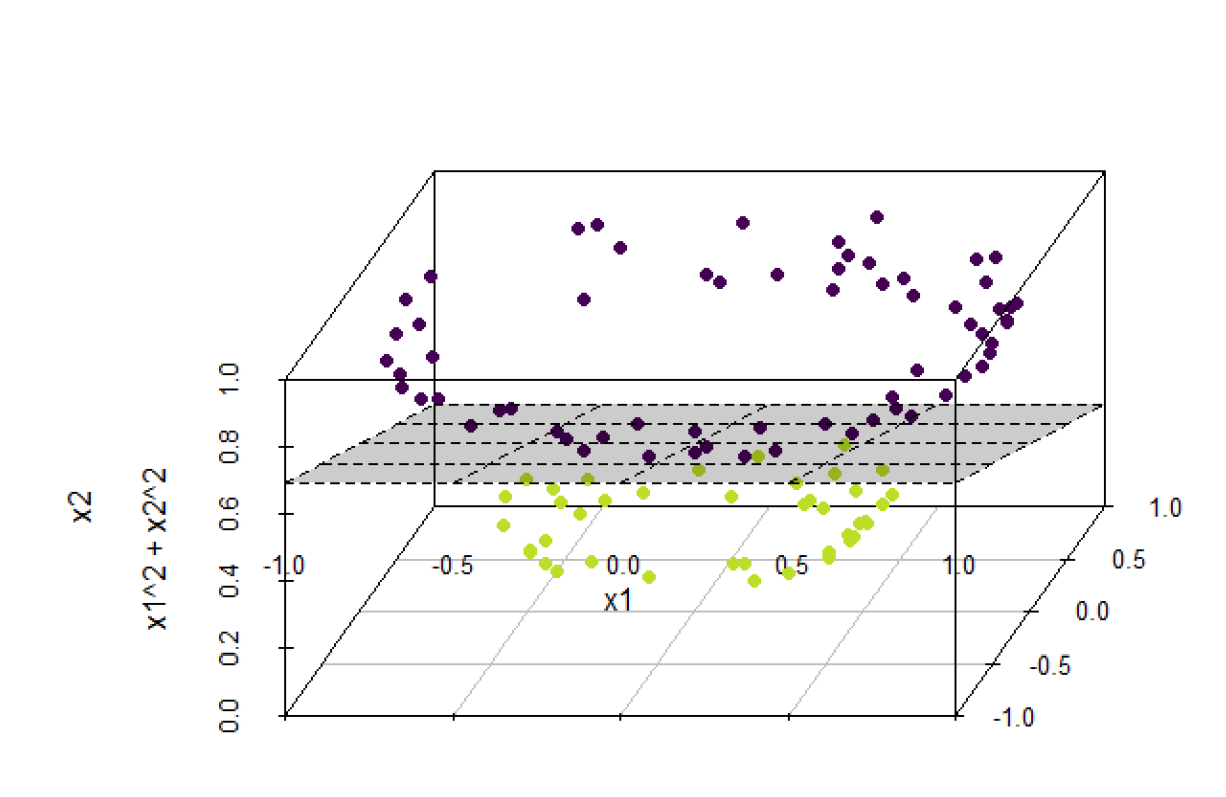
\includegraphics[width=0.9\textwidth]{figure/nonlin_svn_kernel.png}
 \end{minipage}
  \footnotesize
 \begin{minipage}{0.48\textwidth}
 \centering
 % from FCIM 2020 lecture_cim2\2020\09-nonlinear-svm\slides-5-kernel-rbf.Rnw
 $k(\xv, \tilde \xv) = \exp(-\gamma \|\xv - \tilde \xv\|^2)$
 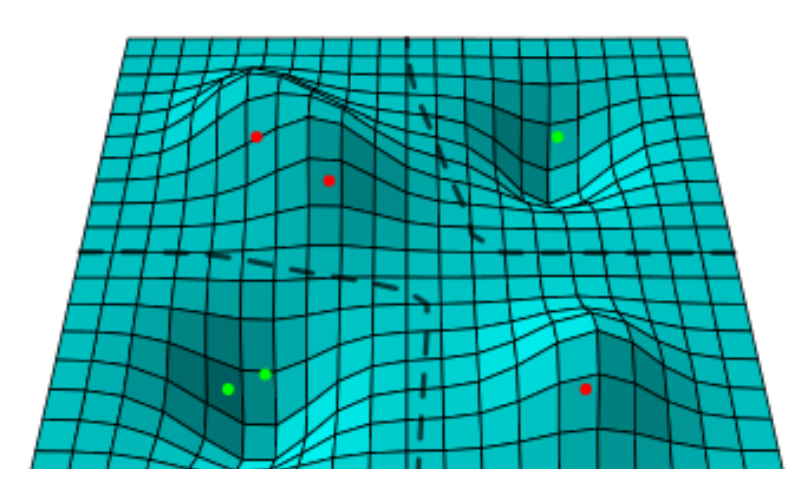
\includegraphics[width=0.95\textwidth]{figure/nonlin-svm-rbf.png}
   
 \end{minipage}

\end{frame}

% ------------------------------------------------------------------------------

\begin{frame}{Non-linear SVM -- Functionality}

\footnotesize

\highlight{Empirical risk}

SVMs can also be interpreted as \textbf{L2-regularized ERM}: 

$$ \frac{1}{2} \|\thetab\|^2 + C \sumin \Lxyi ;\; \Lyf = \max(1-yf, 0),$$ 
with $\Lyf$ as the hinge loss, $\|\thetab\| = 1 / \gamma$ and $C$ as cost parameter for margin violation.

\medskip

\highlight{Optimization} ~~
As the problem is \textbf{not differentiable}, there are the following solutions: 
\begin{enumerate}
\item Use a smoothed loss (squared hinge, huber), then do gradient descent.\\
  NB: Will not  create a sparse SVM if we do not add extra tricks.
\item Use \textbf{subgradient} methods.
\item Do stochastic subgradient descent.\\
  Pegasos: Primal Estimated sub-GrAdient SOlver for SVM.
\end{enumerate}

\medskip


\highlight{Hyperparameters}

\begin{itemize}
  \item \textbf{$C$}: penalization for missclassified data points 
  \item \textbf{Kernel parameters}: depending on which kernel is used (e. g. degree of the polynomial kernel or width of RBF kernel)

\end{itemize}

\medskip

%Support Vector Machine Solvers by Bottou and Lin: https://leon.bottou.org/publications/pdf/lin-2006.pdf
%SVM-optimization and steepest-descent line search by List and Simon: https://www.cs.mcgill.ca/~colt2009/papers/021.pdf
% \highlight{Runtime behavior} ~~ $\mathcal{O}(n^2)$ or $ \mathcal{O}(n^3)$ for $n$ observations depending on the kernel


%\highlight{Runtime behavior} ~~ $\mathcal{O}(n^2 \cdot p + n^3)$ for $n$ 
%observations and $p$ features

\end{frame}

% ------------------------------------------------------------------------------

\begin{frame}{Non-linear SVM -- Pro's \& Con's}

\footnotesize


\begin{columns}[onlytextwidth]
  \begin{column}{0.5\textwidth}
    \highlight{Advantages}
    \footnotesize
    \begin{itemize}
      \positem high \textbf{accuaracy}
      \positem can learn \textbf{non-linear decision boundaries}
      \positem often \textbf{sparse} solution
      \positem robust against overfitting (\textbf{regularized}); especially in high-dimensional space 
      \positem \textbf{stable} solutions, as the non-SV do not influence the separating hyperplane
    \end{itemize}
  \end{column}

  \begin{column}{0.5\textwidth}
    \highlight{Disadvantages}
    \footnotesize
    \begin{itemize}
      \negitem \textbf{costly implementation}; long training times
      \negitem does not scale well to \textbf{larger data sets} \textcolor{blue}{\textbf{??}}
      \negitem only \textbf{linear separation} $\rightarrow$ possible 
      with non-linear SVMs which are explained in the following slides.
      \negitem poor \textbf{interpretability}
      %\item[$\textbf{\textcolor{gray!80}{-}}$] very memory-intensive
      \negitem \textbf{not easy tunable} as it is highly important to choose the right kernel
      
    \end{itemize}
  \end{column}
\end{columns}

\vfill

\small

\conclbox{Non-linear SVMs perform very well for non-linear separable data, but are hard to interpret and need a lot of tuning.}

\end{frame}

% ------------------------------------------------------------------------------

\begin{frame}{Non-linear SVM -- Practical hints}

\footnotesize

  \highlight{Kernels} \\
  \smallskip
 Mainly, these three types of kernels are used: 
 \begin{itemize}
 
 \item \textbf{Linear kernel}: the dot product of the given observations
 
 \item \textbf{Polynomial kernel}: curved lines in the input space
 
 \item \textbf{Radial basis function (RBF) kernel}: complex regions in the input space (e. g. spirals)
 
 \end{itemize}
 
 

\medskip

 \highlight{Tuning} \\
 \begin{itemize}
    \item SVMs are sensitive to its hyperparameters and \textbf{should always be tuned}. 
    \item For the RBF kernel the \textbf{RBF sigma heuristic} is used. 
  \end{itemize}
  

  \medskip

   \highlight{Implementation} 
  \begin{itemize}
    \item \textbf{R:} \code{mlr3} learners \code{LearnerClassifSVM} / 
    \code{LearnerRegrSVM}, calling \code{e1071::svm()}
    \item \textbf{Python:} \code{sklearn.svm.SVC} from package \code{scikit-learn} / package \code{libSVM}
  \end{itemize}

\end{frame}


% ------------------------------------------------------------------------------
% KNN
% ------------------------------------------------------------------------------

\begin{frame}{$k$-nearest neighbors -- Functionality}

\footnotesize

\maketag{Supervised}
\maketag{Non-parametric}
\maketag{White-box}

\medskip

\highlight{General idea}
\begin{itemize}
  \item The \textbf{$k$-nearest neighbors ($k$-NN)} model is based on 
  inter-observational \textbf{distances}, thus heavily depending on the chosen 
  \textbf{distance measure}.
  \item It builds upon the rationale that closeness in feature space infers
  closeness in target space.
  \item The prediction for $\xi$ is the (weighted) \textbf{mean target} 
  (regression) or \textbf{most frequent class} (classification) within 
  its \textbf{$k$-neighborhood} $N_k(\xi)$ (i.e., the $k$ points closest to $\xi$ in
  feature space). \textcolor{blue}{only true for specific loss
  functions???}
\end{itemize}

\medskip
 
\highlight{Hypothesis space} ~~ \textcolor{blue}{step functions over
tesselations of xspace}
$\Hspace = \left\{ \fx \right\}$

\medskip

\highlight{Empirical risk} ~~ Any loss function applicable to 
regression/classification

\highlight{Optimization} ~~ Not necessary

\highlight{Hyperparameters} ~~ Neighborhood size $k$, distance measure

\begin{minipage}{0.5\textwidth}
  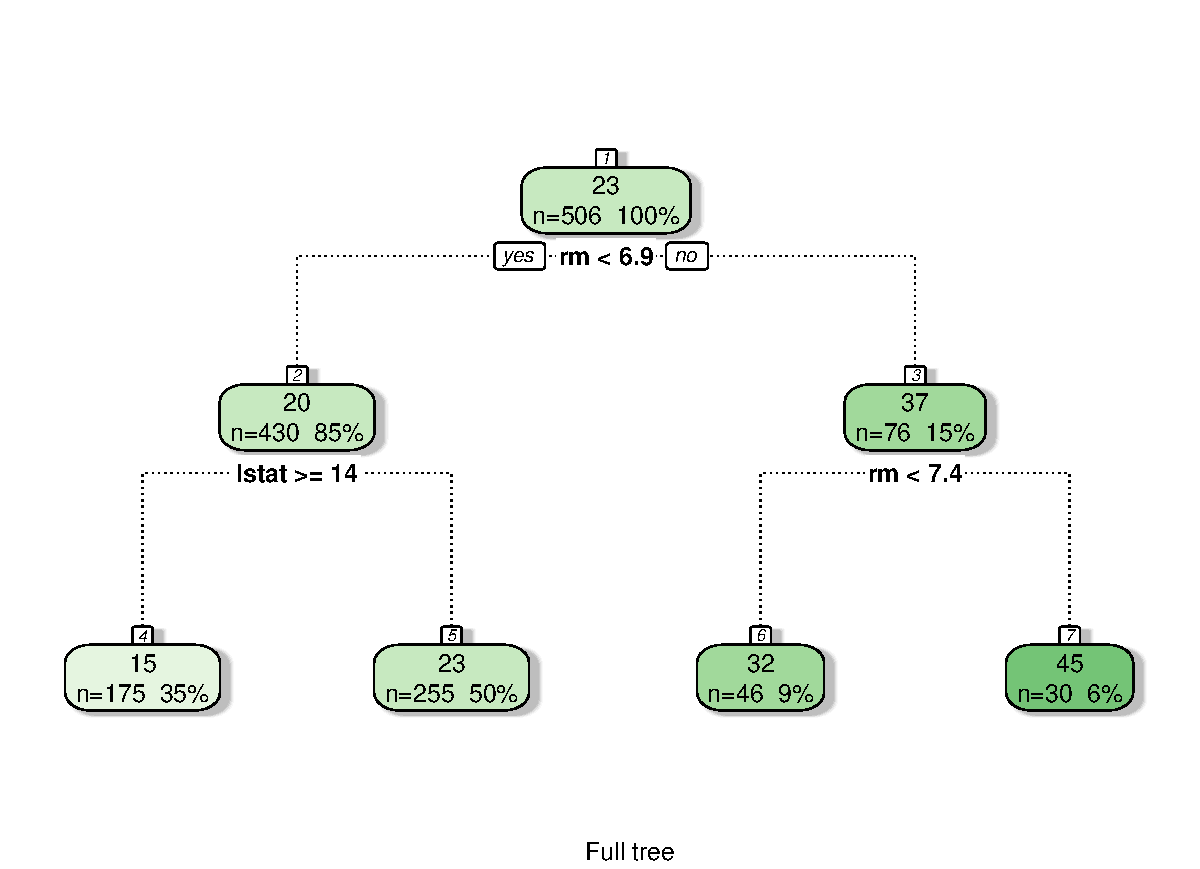
\includegraphics[width=0.9\textwidth]{figure/cart.pdf}
\end{minipage}%
\begin{minipage}{0.5\textwidth}
  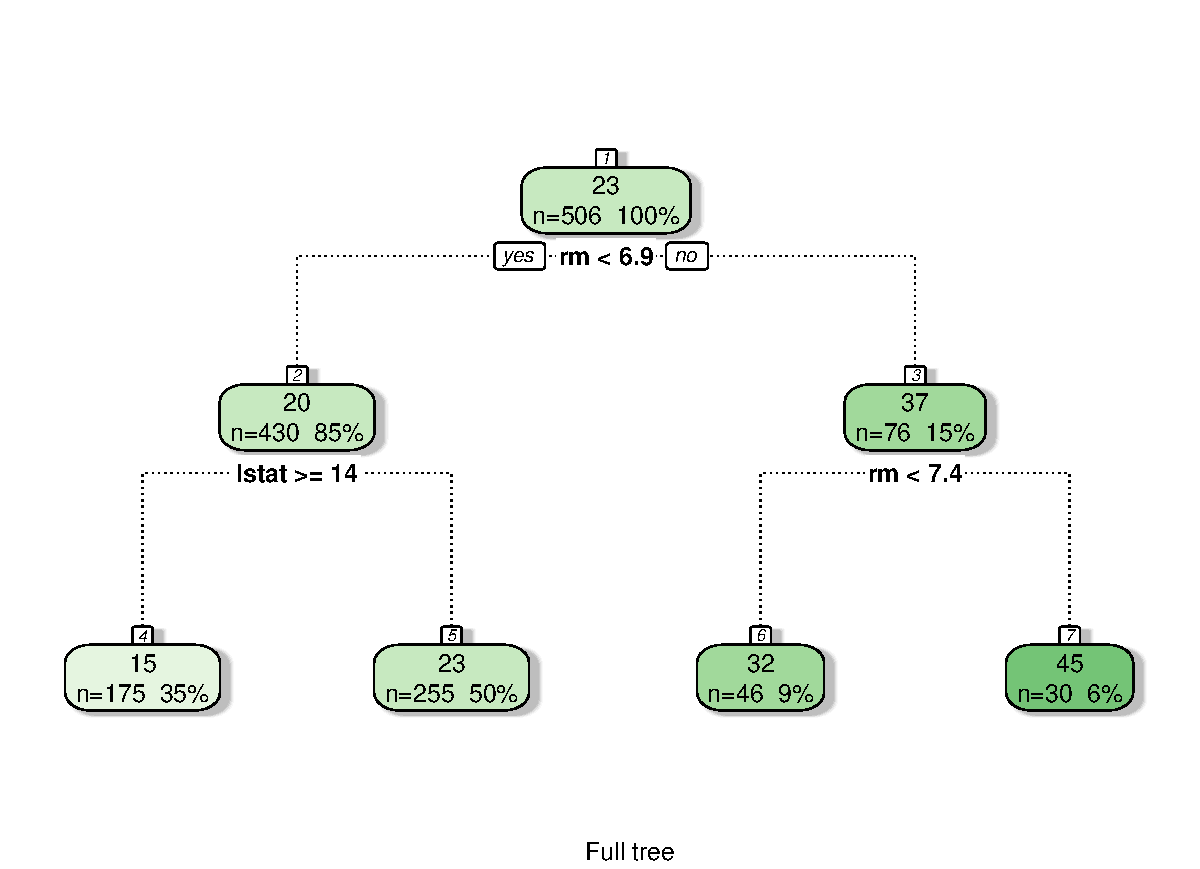
\includegraphics[width=0.9\textwidth]{figure/cart.pdf}
\end{minipage}

\end{frame}

% ------------------------------------------------------------------------------

\begin{frame}{$k$-nearest neighbors -- Pro's \& Con's}

\footnotesize

\begin{columns}[onlytextwidth]
  \begin{column}{0.5\textwidth}
    \highlight{Advantages}
    \footnotesize
    \begin{itemize}
      \positem \textbf{Easy} 
    \end{itemize}
  \end{column}
  \begin{column}{0.5\textwidth}
    \highlight{Disadvantages}
    \footnotesize
    \begin{itemize}
      \negitem Rather 
    \end{itemize}
  \end{column}
\end{columns}

\vfill

\small

\conclbox{Foo}

\end{frame}

% ------------------------------------------------------------------------------

\begin{frame}{$k$-nearest neighbors -- Practical hints}

\footnotesize

\highlight{Neighborhood size}

Unless 

\medskip

\highlight{Distance measures}

Unless 

\medskip

\highlight{Neighborhoods in higher dimensions}

Unless 

\medskip

\highlight{Implementation}
\begin{itemize}
  \item \textbf{R:} \code{mlr3} learners \code{LearnerClassifKKNN} /
  \code{LearnerRegrKKNN}, calling \code{kknn::kknn()}
  \item \textbf{Python:} \code{KNeighborsClassifier} / 
  \code{KNeighborsRegressor} from package \code{scikit-learn}
  \item While optimization per se is not necessary, efficiency of distance 
  computation can be improved.
\end{itemize}

\medskip

\highlight{Bagging / boosting} 

Since 

\end{frame}

% ------------------------------------------------------------------------------
% CART (Classification and Regression Trees)
% ------------------------------------------------------------------------------

\begin{frame}{CART -- Functionality}

\footnotesize

\maketag{Supervised}
\maketag{Non-parametric}
\maketag{White-box}
\maketag{Feature selection}

\medskip

\highlight{General idea}
\begin{itemize}
  \item Starting from a root node, \textbf{classification \& regression trees 
  (CART)} perform repeated \textbf{binary splits} of the data according to feature 
  values, thereby subsequently dividing the input space $\Xspace$ into $T$ 
  \textbf{rectangular partitions} $Q_t$.
  \item Observations are passed along until each ends up in exactly one leaf 
  node (unless \textbf{stopped early} or \textbf{pruned}).
  \item In each step, CART find the optimal feature-threshold combination to 
  split by.
  \item Leaf node $t$ is assigned response $c_t$.
\end{itemize}

\medskip
 
\highlight{Hypothesis space} ~~
$\Hspace = \left\{ \fx: \fx = \sum_{t = 1}^T c_t \I(\xv \in Q_t) 
\right\}$

\medskip

\begin{minipage}{0.5\textwidth}
  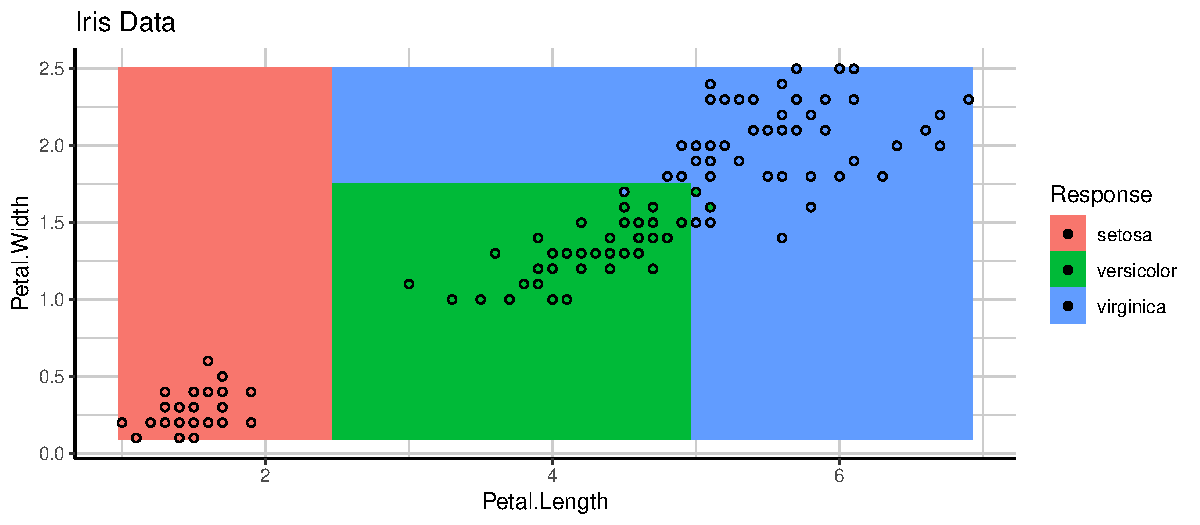
\includegraphics[width=\textwidth]{figure/cart-partition}
\end{minipage}%
\begin{minipage}{0.5\textwidth}
  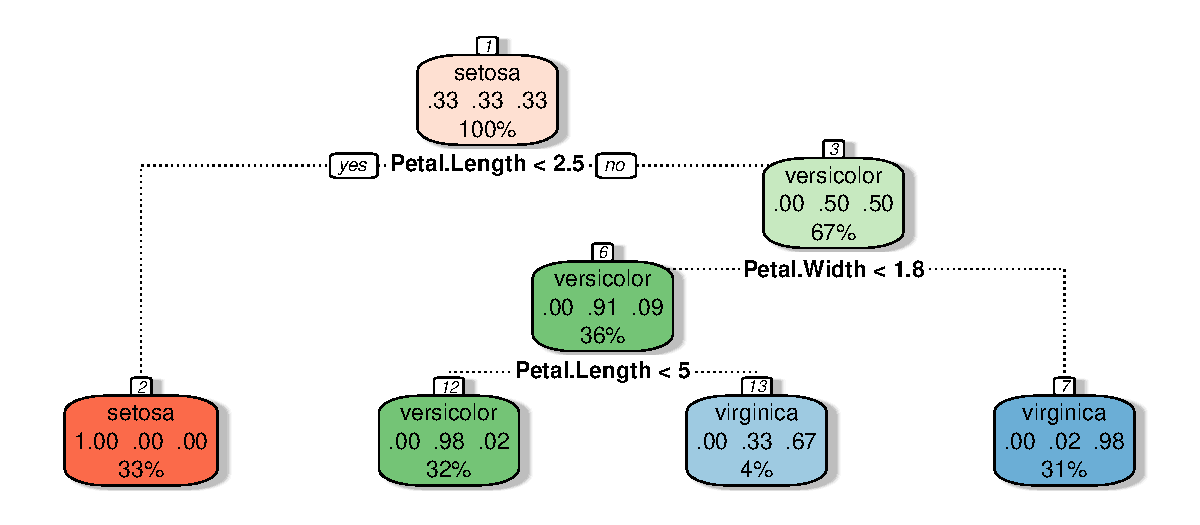
\includegraphics[width=\textwidth]{figure/cart-tree}
\end{minipage}
\begin{minipage}{0.5\textwidth}
  \tiny Prediction surface for \code{iris} data, 3 splits 
\end{minipage}%
\begin{minipage}{0.5\textwidth}
  \tiny Corresponding classification tree
\end{minipage}

\end{frame}

% ------------------------------------------------------------------------------

\begin{frame}{CART -- Functionality}

\footnotesize

\highlight{Empirical risk} \\

\begin{itemize}
  \item Empirical risk is calculated for each potential terminal node $\Np_t$
  of a split.
  \item In general, trees can handle any type of loss function. Typical choices
  are:
  \begin{itemize}
    \footnotesize
    \item Classification (for $g$ classes):
    \begin{itemize}
      \footnotesize
      \item Using \textbf{Brier score} ~~
      $\risk(\Np_t) = \sum\limits_{(\xv,y) \in \Np_t} \sumkg \left( \I(y = k)
      - \pikx \right)^2$
      \item Using \textbf{Bernoulli loss} ~~
      $\risk(\Np_t) = \sum\limits_{(\xv,y) \in \Np_t} \sumkg \I(y = k) \cdot
      \log(\pikx)$
    \end{itemize}
    \item Regression: Using \textbf{quadratic loss} ~~
    $\risk(\Np_t) = \sum\limits_{(\xv,y) \in \Np_t} (y - c_t)^2$
  \end{itemize}
\end{itemize}

\medskip

\highlight{Optimization}

\textbf{Exhaustive} search over all (randomly selected) split candidates in each 
node to minimize empirical risk in the child nodes (greedy optimization)

\medskip

\highlight{Hyperparameters} ~~ \textbf{Complexity}, i.e., 
number of leaves $T$ \\

\medskip

% \highlight{Runtime behavior} ~~ $\mathcal{O}(n^2 \cdot p)$ for $n$ 
% observations and $p$ features

\normalsize
  
\end{frame}

% ------------------------------------------------------------------------------

\begin{frame}{CART -- Pro's \& Con's}

\footnotesize

\begin{columns}[onlytextwidth]
  \begin{column}{0.5\textwidth}
    \highlight{Advantages}
    \footnotesize
    \begin{itemize}
      \positem \textbf{Easy} to understand, interpret \& visualize
      \positem Automatic handling of \textbf{non-numerical} features
      \positem Built-in \textbf{feature selection}
      \positem Automatic handling of \textbf{missings} 
      \positem \textbf{Interaction} effects between features easily possible, 
      even of higher orders
      \positem \textbf{Fast} computation and good scalability
      \positem High \textbf{flexibility} (custom split criteria or leaf-node 
      prediction rules)   
    \end{itemize}
  \end{column}
  \begin{column}{0.5\textwidth}
    \highlight{Disadvantages}
    \footnotesize
    \begin{itemize}
      \negitem Rather \textbf{low accuracy} (at least, without bagging or 
      boosting)
      \negitem High \textbf{variance/instability}: strong dependence on training 
      data
      \negitem Therefore, poor generalization \& risk of \textbf{overfitting}
      \negitem Several steps required for modeling \textbf{linear} relationships
      \negitem In presence of categorical features, \textbf{bias} towards 
      features with \textbf{many categories}
    \end{itemize}
  \end{column}
\end{columns}

\vfill

\small

\conclbox{Simple and good with feature selection, but not the best predictor}

\end{frame}

% ------------------------------------------------------------------------------

\begin{frame}{CART -- Practical hints}

\footnotesize

\highlight{Pruning / early stopping}

Unless interrupted, splitting will go on until each leaf node contains a single 
observation (expensive + overfitting!) \\
\smallskip
$\rightarrow$ Use \textbf{pruning} and \textbf{stopping criteria} to limit 
complexity

\medskip

\highlight{Implementation}
\begin{itemize}
  \item \textbf{R:} \code{mlr3} learners \code{LearnerClassifRpart} / 
    \code{LearnerRegrRpart}, calling \code{rpart::rpart()}
  \item \textbf{Python:} \code{DecisionTreeClassifier} / 
  \code{DecisionTreeRegressor} from package \code{scikit-learn}
  \item Complexity controlled via tree depth, minimum number of observations 
  per node, maximum number of leaves, minimum risk reduction per split, ...
\end{itemize}

\medskip

\highlight{Bagging / boosting} 

Since CART are instable predictors on their own, they are typically ensembled
to form a \textbf{random forest} (\textbf{bagging}) or used in combination with 
\textbf{boosting}.

\end{frame}

% ------------------------------------------------------------------------------
% RANDOM FORESTS
% ------------------------------------------------------------------------------

\begin{frame}{Random Forest -- Functionality}

\footnotesize

\maketag{SUPERVISED}
\maketag{NON-PARAMETRIC}
\maketag{BLACK-BOX}
\maketag{FEATURE SELECTION}

\medskip

\highlight{General idea} 
\begin{itemize}
  \item \textbf{Random forests (RF)} perform \textbf{bagging}: they combine 
  $M$ trees (base learners) to form a strong \textbf{ensemble} learner. 
  \item They use \textbf{complex} trees with low  bias and compensate for the
  resulting variance by aggregating them in a \textbf{decorrelated} manner. 
  \item Each tree is trained on a \textbf{bootstrap sample} of the data and 
  only on a random \textbf{subset of features} to incur variability.
  \item Aggregation via \textbf{averaging} (regression) or 
  \textbf{majority voting} (classification).
\end{itemize}

\medskip

\highlight{Hypothesis space} ~~
$\Hspace = \left\{ \fx: \fx = \frac{1}{M} \sum_{m = 1}^M \sum_{t = 1}^{T^{[m]}} 
c_t^{[m]} \I(\xv \in Q_t^{[m]}) \right\}$

\medskip

\begin{minipage}{0.5\textwidth}
  % FIGURE SOURCE: https://docs.google.com/presentation/d/1xodP6ayu1Gay6mMKgzVWYEFmSoeG5kNuqsaTkFFmd78  /edit
  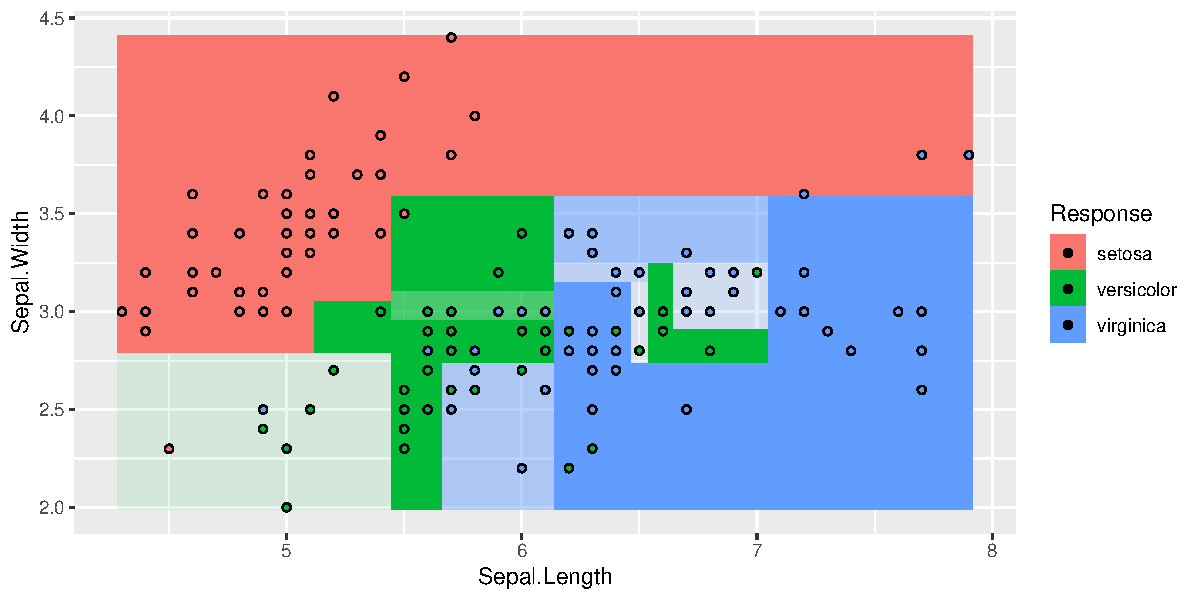
\includegraphics[width=\textwidth]{figure/rf-10}
\end{minipage}%
\begin{minipage}{0.5\textwidth}
  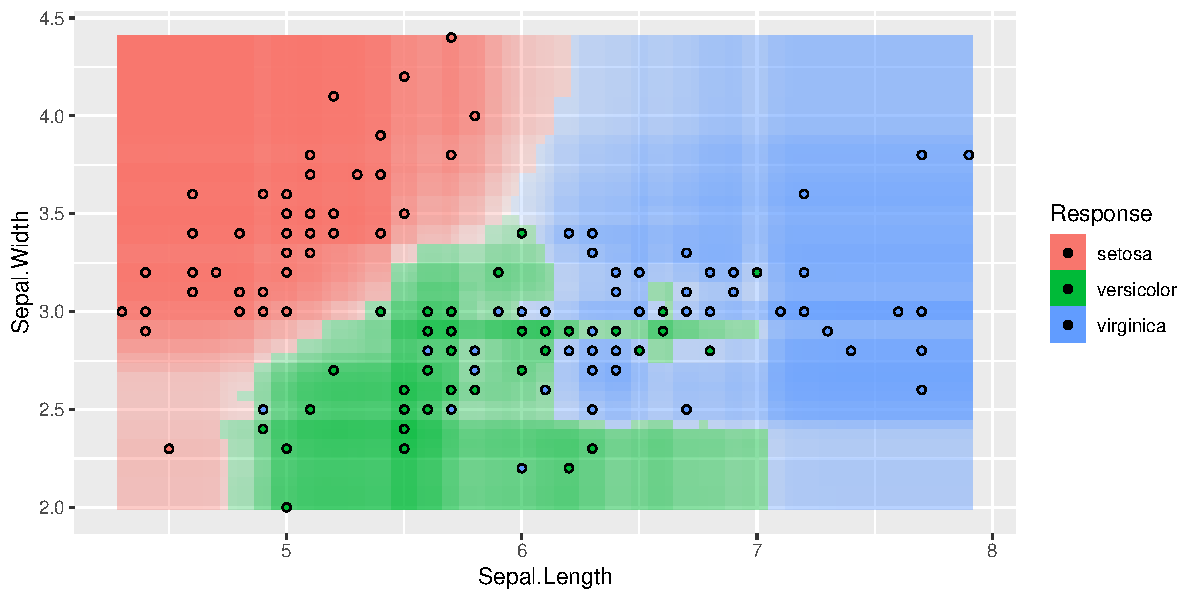
\includegraphics[width=\textwidth]{figure/rf-500}
\end{minipage}
\begin{minipage}{0.5\textwidth}
  \tiny Prediction surface for \code{iris} data with a single tree
\end{minipage}%
\begin{minipage}{0.5\textwidth}
  \tiny Prediction surface for \code{iris} data with 500-tree ensemble
\end{minipage}

\end{frame}

% ------------------------------------------------------------------------------

\begin{frame}{Random Forest -- Functionality}

\footnotesize

\highlight{Empirical risk}

\begin{itemize}
  \item Applicable with \textbf{any} kind of loss function (just like tree base 
  learners)
  \item Computation of empirical risk for all potential child nodes in all trees
\end{itemize}

\medskip

\highlight{Optimization}

\textbf{Exhaustive} search over
all (randomly selected) split candidates in each node of each tree to minimize
empirical risk in the child nodes (greedy optimization) \\

\medskip

\highlight{Hyperparameters}

\begin{itemize}
  \item \textbf{Ensemble size}, i.e., number of trees
  \item \textbf{Complexity}, i.e., number of leaves $T$ of each base learner
  \item \textbf{Number of split candidates}, i.e., number of features to be
  considered as splitting variables at each split \\
  $\rightarrow$ Frequently used heuristics: 
  $\left \lfloor{\sqrt{p}}\right \rfloor$ for classification and
  $\left \lfloor{p/3}\right \rfloor$ for regression
\end{itemize}

\medskip

% \highlight{Runtime behavior} ~~
% $\mathcal{O}(M \cdot n^2 \cdot p)$ for $M$ trees, $n$ observations and $p$ 
% features
  
\end{frame}


% ------------------------------------------------------------------------------

\begin{frame}{Random Forest -- Pro's \& Con's}

\footnotesize

\begin{columns}[onlytextwidth]
  \begin{column}{0.5\textwidth}
    \highlight{Advantages}
    \footnotesize
    \begin{itemize}
      \positem Translation of most of \textbf{base learners'} advantages (e.g., 
      inherent variable selection, handling of missing data)
      \positem Fairly good at \textbf{prediction}: improved accuracy through 
      bagging
      \positem Inherent computation of \textbf{feature importance}
      \positem Quite \textbf{stable} wrt changes in the data
      \positem Good with \textbf{high-dimensional} data, even in presence of 
      noisy covariates
      \positem Applicable to \textbf{unbalanced} data
      \positem Easy to \textbf{parallelize}
      \positem Rather easy to \textbf{tune}
    \end{itemize}
  \end{column}
  \begin{column}{0.5\textwidth}
    \highlight{Disadvantages}
    \footnotesize
    \begin{itemize}
      \negitem Translation of some of \textbf{base learners'} disadvantages 
      (e.g., trouble to model linear relations, bias towards features with many 
      categories)
      \negitem Loss of single trees' \textbf{interpretability} -- black-box 
      method
      \negitem Hard to \textbf{visualize}
      \negitem Often suboptimal for \textbf{regression}
      \negitem Often still inferior in \textbf{performance} to other methods 
      (e.g., boosting)
    \end{itemize}
  \end{column}
\end{columns}

\vfill

\small

\conclbox{Fairly good predictor, but black-box method}

\end{frame}

% ------------------------------------------------------------------------------

\begin{frame}{Random Forest -- Practical hints}

\footnotesize

\highlight{Pre-processing} 

Inherent feature selection of random forests, but high \textbf{computational 
costs} for large number of features \\
$\rightarrow$ Upstream feature selection (e.g., via PCA) might be advisable
\lz

\highlight{Implementation}

\begin{itemize}
  \item \textbf{R:} \code{mlr3} learners \code{LearnerClassifRanger} / 
    \code{LearnerRanger}, calling \code{ranger::ranger()}
  \item \textbf{Python:} \code{RandomForestClassifier} / 
  \code{RandomForestRegressor} from package \code{scikit-learn}
\end{itemize}

\medskip

\highlight{Tuning} 

\begin{itemize}
  \item Overall \textbf{limited tunability}
  \item Number of split candidates often more impactful than number of trees
\end{itemize}

\end{frame}

% ------------------------------------------------------------------------------
% GRADIENT BOOSTING
% ------------------------------------------------------------------------------

\begin{frame}{Gradient Boosting -- Functionality}

\footnotesize

\maketag{supervised}
\maketag{NON-PARAMETRIC}
\maketag{BLACK-BOX}
\maketag{FEATURE SELECTION}

\medskip

\highlight{General idea}

\begin{itemize}
  \item \textbf{Gradient boosting (GB)} is an \textbf{ensemble} method that 
  constructs a strong learner from weak base learners (frequently, CART).
  \item As opposed to \textbf{bagging}, however, base learners are assembled in a 
  \textbf{sequential, stage-wise} manner: in each iteration, GB improves the 
  current model by adding a new component that minimizes empirical risk.
  \item Each base learner is fitted to the current \textbf{point-wise residuals} 
  \\ $\rightarrow$ One boosting iteration $\widehat{=}$ one approximate 
  \textbf{gradient step in function space}
  \item The final model is a weighted sum of base learners $b(\xv, \thetam)$ 
  with weights $\betam$.
\end{itemize}

\medskip

\highlight{Hypothesis space} ~~
$\Hspace = \left\{ \fx: \fx = \sum_{m = 1}^M \betam b(\xv, \thetam) \right\}$

\begin{minipage}{0.5\textwidth}
  % FIGURE SOURCE: http://arogozhnikov.github.io/2016/06/24/gradient_boosting_explained.html
  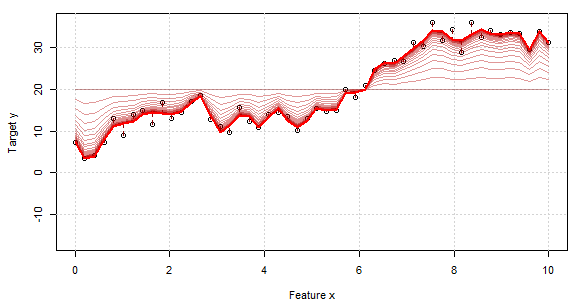
\includegraphics[width=0.8\textwidth]{figure/gb}
\end{minipage}%
\begin{minipage}{0.5\textwidth}
  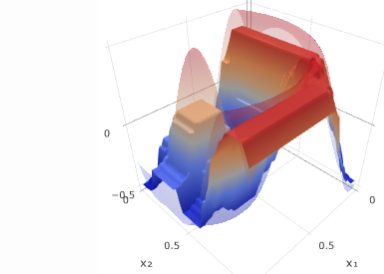
\includegraphics[width=0.6\textwidth]{figure/gb_3d}
\end{minipage}
\begin{minipage}{0.5\textwidth}
  \tiny Gradient boosting for univariate function \textcolor{blue}{WHICH FIGURE}
\end{minipage}%
\begin{minipage}{0.5\textwidth}
  \tiny Gradient boosting for bivariate function \textcolor{blue}{WHICH FIGURE}
\end{minipage}

\end{frame}

% ------------------------------------------------------------------------------

\begin{frame}{Gradient Boosting -- Functionality}

\footnotesize

\highlight{Empirical risk}

\begin{itemize}
  \item \textbf{Outer loss:} Loss used to compute pseudo-residuals -- how large 
  is the error of the current model fit? \\
  $\rightarrow$ Arbitrary \textbf{differentiable} loss function
  \item \textbf{Inner loss:} Loss used to fit next base learner component to 
  current pseudo-residuals \\
  $\rightarrow$ Typically, \textbf{quadratic loss} (desirable 
  optimization properties)
\end{itemize}

\medskip

\highlight{Optimization} ~~ \textbf{Functional gradient descent} for outer 
optimization loop, procedure for inner one depending on inner loss

\medskip

\highlight{Hyperparameters}

\begin{itemize}
  \item \textbf{Ensemble size}, i.e., number of base learners
  \item \textbf{Learning rate}, i.e., impact of single base learner
  \item \textbf{Complexity} of base learners (depending on type used)
\end{itemize}

\medskip

% \highlight{Runtime behavior} ~~ $\mathcal{O}(M \cdot n \cdot p)$ 
% for $M$ base learners, $n$ observations and $p$ features

\end{frame}

% ------------------------------------------------------------------------------

\begin{frame}{Gradient Boosting -- Pro's \& Con's}

\footnotesize

\begin{columns}[onlytextwidth]
  \begin{column}{0.5\textwidth}
    \highlight{Advantages}
    \footnotesize
    \begin{itemize}
      \positem Powerful \textbf{off-the-shelf} method for supercharging weak 
      learners' performance
      \positem Translation of most of \textbf{base learners'} advantages 
      (e.g., for tree boosting: inherent 
      variable selection, handling of missing data)
      \positem High predictive \textbf{accuracy} that is hard to outperform
      \positem High \textbf{flexibility} (custom loss functions, many tuning 
      options) 
      \positem Applicable to \textbf{unbalanced} data
    \end{itemize}
  \end{column}
  \begin{column}{0.5\textwidth}
    \highlight{Disadvantages}
    \footnotesize
    \begin{itemize}
      \negitem Hardly \textbf{interpretable} -- black-box method
      \negitem Hard to \textbf{visualize}
      \negitem Prone to \textbf{overfitting}
      \negitem Sensitive to \textbf{outliers}
      \negitem Hard to \textbf{tune} (high sensitivity to variations in 
      hyperparameter values)
      \negitem Rather \textbf{slow} in training
      \negitem Hard to \textbf{parallelize}
    \end{itemize}
  \end{column}
\end{columns}

\vfill

\small

\conclbox{High-performing predictor, but rather delicate to handle}

\end{frame}

% ------------------------------------------------------------------------------

\begin{frame}{Gradient Boosting -- Practical hints}

\footnotesize

\highlight{XGBoost (extreme gradient boosting)} 

Fast, efficient implementation of gradient-boosted decision trees that has
become \textbf{state of the art} for many machine learning problems \\
$\rightarrow$ Clever modeling techniques + computational speed \\

\medskip

\highlight{Stochastic gradient boosting (SGB)}

Faster, approximate version of GB that performs each iteration only on 
\textbf{random subset} of the data \\

\medskip

\highlight{Implementation}

\begin{itemize}
  \item \textbf{R:} \code{mlr3} learners \code{LearnerClassifXgboost} / 
  \code{LearnerXgboost}, calling \code{xgboost::xgb.train()}
  \item \textbf{Python:} \code{GradientBoostingClassifier} / 
  \code{GradientBoostingRegressor} from package \code{scikit-learn}, 
  \code{XGBClassifier} / \code{XGBRegressor} from package \code{xgboost}
\end{itemize}

\medskip

\highlight{Tuning}
\begin{itemize}
  \item Overall \textbf{limited tunability}
  \item Number of split candidates often more impactful than number of trees
\end{itemize}

\end{frame}

% ------------------------------------------------------------------------------
% NEURAL NETWORK
% ------------------------------------------------------------------------------

\begin{frame}{Neural Network -- Functionality}

\footnotesize

\maketag{|UN| SUPERVISED}
\maketag{|Non| parametric}
\maketag{BLACK-BOX}

\medskip

\highlight{General idea}
\begin{itemize}
  \item A \textbf{neural network (NN)} is a model architecture loosely inspired by 
  the human brain. It consists of various \textbf{neurons}, organized in 
  \textbf{layers} assembled through weighted functional connections. 
  \item Batches of data enter in the \textbf{input layer} and sequentially pass 
  through $h$ \textbf{hidden layers}, each of which performs a linear 
  \textbf{transformation} $\phi^{(j)}$and a non-linear \textbf{activation} 
  $\sigma^{(j)}$, thus creating intermediary representations of the data.
  \item The \textbf{output layer} yields predictions after a final transformation $\phi $ and 
  scaling $\tau$.
  \item The resulting loss is used to update the weights for the next 
  \textbf{epoch}.
\end{itemize}

\medskip
 
\highlight{Hypothesis space} ~~
$$\Hspace = \left\{ \fx: \fx = \tau \circ \phi \circ \sigma^{(h)} \circ
\phi^{(h)} \circ \sigma^{(h - 1)} \circ \phi^{(h - 1)} \circ ... \circ 
\sigma^{(1)} \circ \phi^{(1)} (\xv) \right\}$$

\medskip

\begin{minipage}{0.33\textwidth}
  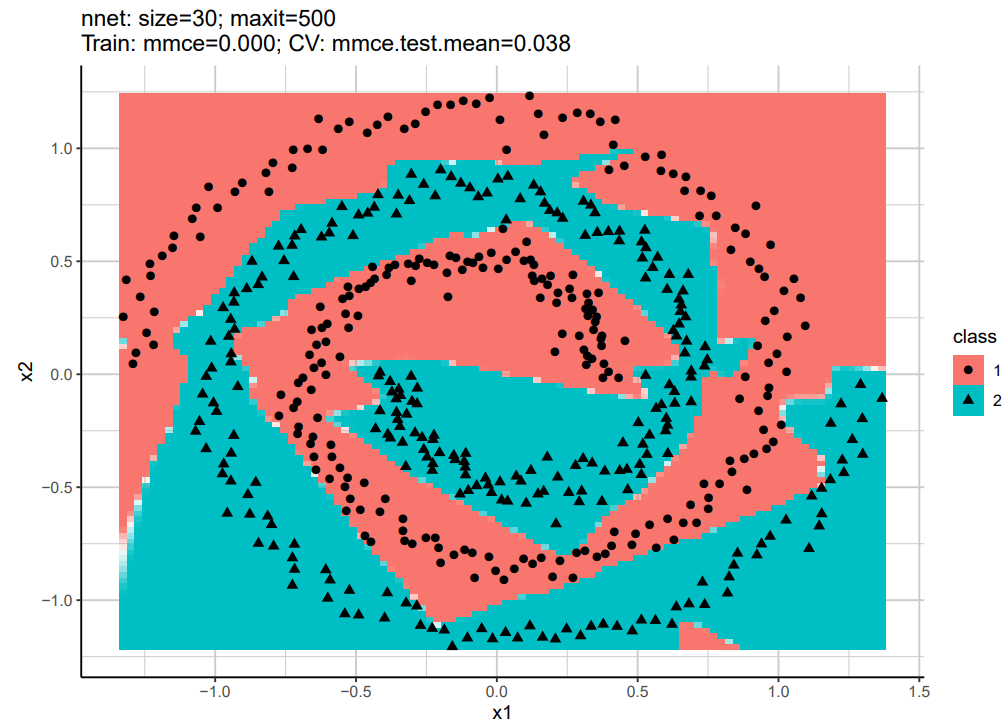
\includegraphics[width=0.7\textwidth]{figure/nn-decision-regions}
\end{minipage}%
\begin{minipage}{0.33\textwidth}
  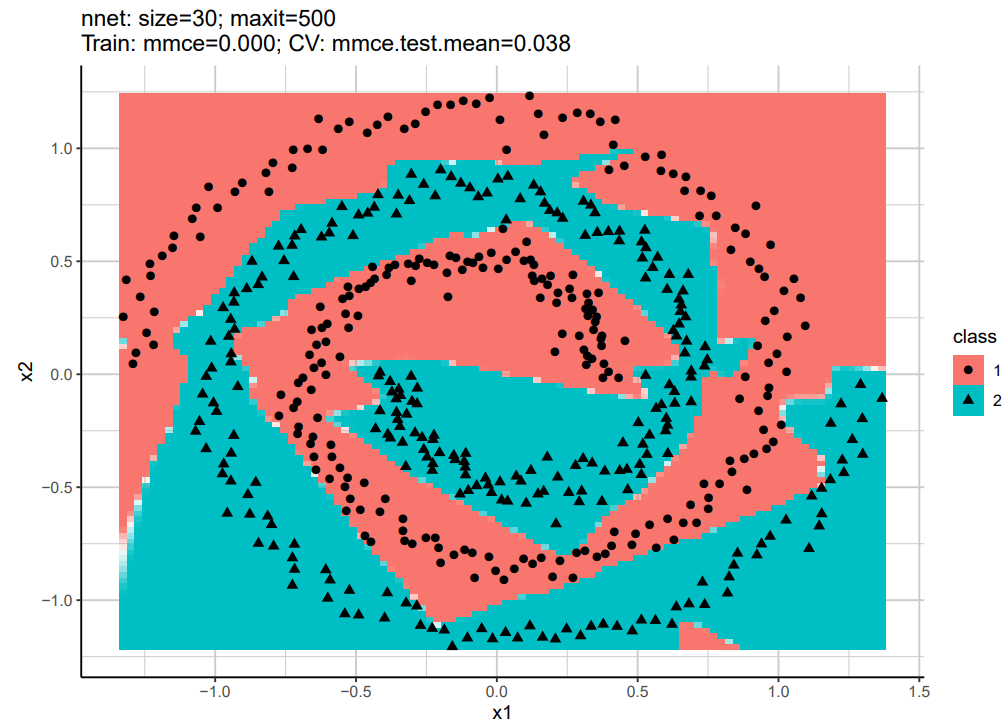
\includegraphics[width=0.7\textwidth]{figure/nn-decision-regions}
\end{minipage}%
\begin{minipage}{0.33\textwidth}
  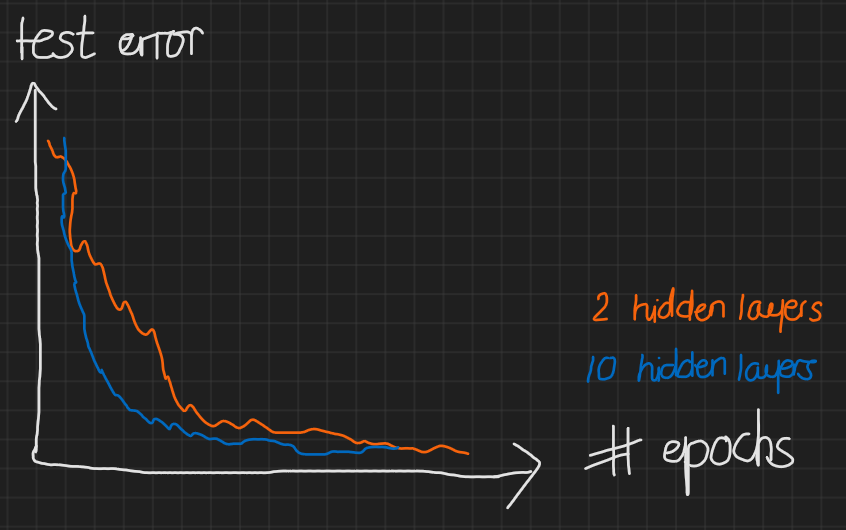
\includegraphics[width=0.6\textwidth]{figure/nn-mmce-epochs}
\end{minipage}
\begin{minipage}{0.67\textwidth}
  \tiny \textcolor{blue}{Classification of \code{spirals} data with X \& Y 
  layers/epochs}
\end{minipage}%
\begin{minipage}{0.33\textwidth}
  \tiny \textcolor{blue}{Classification error vs layers/epochs}
\end{minipage}

\end{frame}

% ------------------------------------------------------------------------------

\begin{frame}{Neural Network -- Functionality}

\footnotesize

\highlight{Empirical risk} ~~
\textcolor{blue}{Any \textbf{differentiable} loss function}

\medskip

\highlight{Optimization}

NNs are optimized by \textbf{backpropagation} which consists of two steps:
\begin{itemize}
  \item \textbf{Forward pass}: Predict result with current weights and 
  compute empirical risk according to chosen loss function. 
  \item \textbf{Backward pass}: Calculate error contribution of each weight by 
  means of gradient descent -- which essentially means applying the chain rule
  to the composition of functions applied in each layer -- and update weights 
  accordingly. 
\end{itemize}

\medskip

\highlight{Hyperparameters}

\begin{itemize}
  \item Number of hidden \textbf{layers} (depth), number of \textbf{neurons} 
  per layer
  \item \textbf{Activation} function(s)
  \item \textbf{Learning rate} for backpropagation
  \item Number of iterations (\textbf{epochs}), \textbf{batch} size
  \item Initial \textbf{weights} 
  \item ...
\end{itemize}

\medskip

% \highlight{Runtime behavior} ~~ \textcolor{blue}{???}

\end{frame}

% ------------------------------------------------------------------------------

\begin{frame}{Neural Network -- Pro's \& Con's}

\footnotesize

\begin{columns}[onlytextwidth]
  \begin{column}{0.5\textwidth}
    \highlight{Advantages}
    \footnotesize
    \begin{itemize}
      \positem Able to solve \textbf{complex, non-linear} regression or 
      classification problems
      \positem Therefore, typically very good \textbf{performance}
      \positem Built-in \textbf{feature extraction} - obtained by intermediary
      representations
      \positem Suitable for \textbf{unstructured} data (e. g. image, audio, 
      text data)
      \positem Easy handling of \textbf{high-dimensional} or \textbf{missing} 
      data
      \positem \textbf{Parallelizable} structure
    \end{itemize}
  \end{column}

  \begin{column}{0.5\textwidth}
    \highlight{Disadvantages}
    \footnotesize
    \begin{itemize}
      \negitem Computationally \textbf {expensive} \\
      $\rightarrow$ slow to train and forecast
      \negitem Large \textbf{amounts} of data required 
      \negitem \textbf{Faster-than-linear} scaling of weight matrices with 
      increased network size 
      \negitem Network architecture requiring much \textbf{expertise} in tuning
      \negitem \textbf{Black-box} model -- hard to interpret or explain
      \negitem Tendency towards \textbf{overfitting}
      
    \end{itemize}
  \end{column}
\end{columns}

\vfill

\small

\conclbox{Able to learn extremely complex functions, but computationally 
expensive and hard to get right}

\end{frame}

% ------------------------------------------------------------------------------

\begin{frame}{Neural Network -- Practical hints}

\footnotesize

\highlight{Types of neural networks (RNNs, CNNs)}

\begin{itemize}
  \item \textbf{Recurrent neural networks (RNNs}: Deep NN that make use of 
  \textbf{sequential} information with temporal \textbf{dependencies} \\
  $\rightarrow$ Frequently applied to \textbf{natural language processing}
  \item \textbf{Convolutional neural networks (CNNs)}: Regularized version of the 
  fully connected feed-forward NN (where each neuron is connected to all 
  neurons of the subsequent layer) that abstracts inputs to feature maps via 
  \textbf{convolution} \\
  $\rightarrow$ Frequently applied to \textbf{image recognition}

\end{itemize}

\medskip

\highlight{Problem of neural architecture search (NAS)}

NN are \textbf{not off-the-shelf} methods -- the network architecture needs to 
be tailored to each problem anew \\
$\rightarrow$ Automated machine learning attempts to learn architectures

\medskip
 
\highlight{Implementation}

\begin{itemize}
  \item \textbf{R:} package \code{neuralnet}
  \item \textbf{Python:} libraries \code{PyTorch}, \code{keras}
\end{itemize}

\end{frame}

% % ------------------------------------------------------------------------------
% 
% % 
% % % ------------------------------------------------------------------------------
% % % KNN 
% % % ------------------------------------------------------------------------------
% 
% \LARGE
% \begin{frame}{\textcolor{gray!80}{KNN} ~~ Functionality}
% \normalsize
% \vspace{-0.5cm}
% \noindent \textcolor{gray!80}{\rule{\textwidth}{1pt}}
% 
% \vspace{0.3cm}
% 
% \footnotesize
% 
% \colorbox{gray!80}{\textcolor{white}{SUPERVISED}}
% \colorbox{gray!80}{\textcolor{white}{PARAMETRIC}}
% \colorbox{gray!80}{\textcolor{white}{WHITE-BOX}}
% %\colorbox{gray!80}{\textcolor{white}{REGRESSION}}
% %\colorbox{gray!80}{\textcolor{white}{FEATURE SELECTION}}
% 
% \medskip
% 
% \textbf{\textcolor{gray!80}{General idea}} ~~
% \begin{itemize}
% 
% \item XX
% 
% \end{itemize}
% 
% \medskip
% 
% \textbf{\textcolor{gray!80}{Hypothesis space}} ~~
% %$\Hspace = \{ \theta_0 + \thx\ |\ (\theta_0, \thetab) \in \R^{p+1} \} $
% 
% \medskip
% % \footnotesize
% % \begin{minipage}{0.5\textwidth}
% \centering
%   %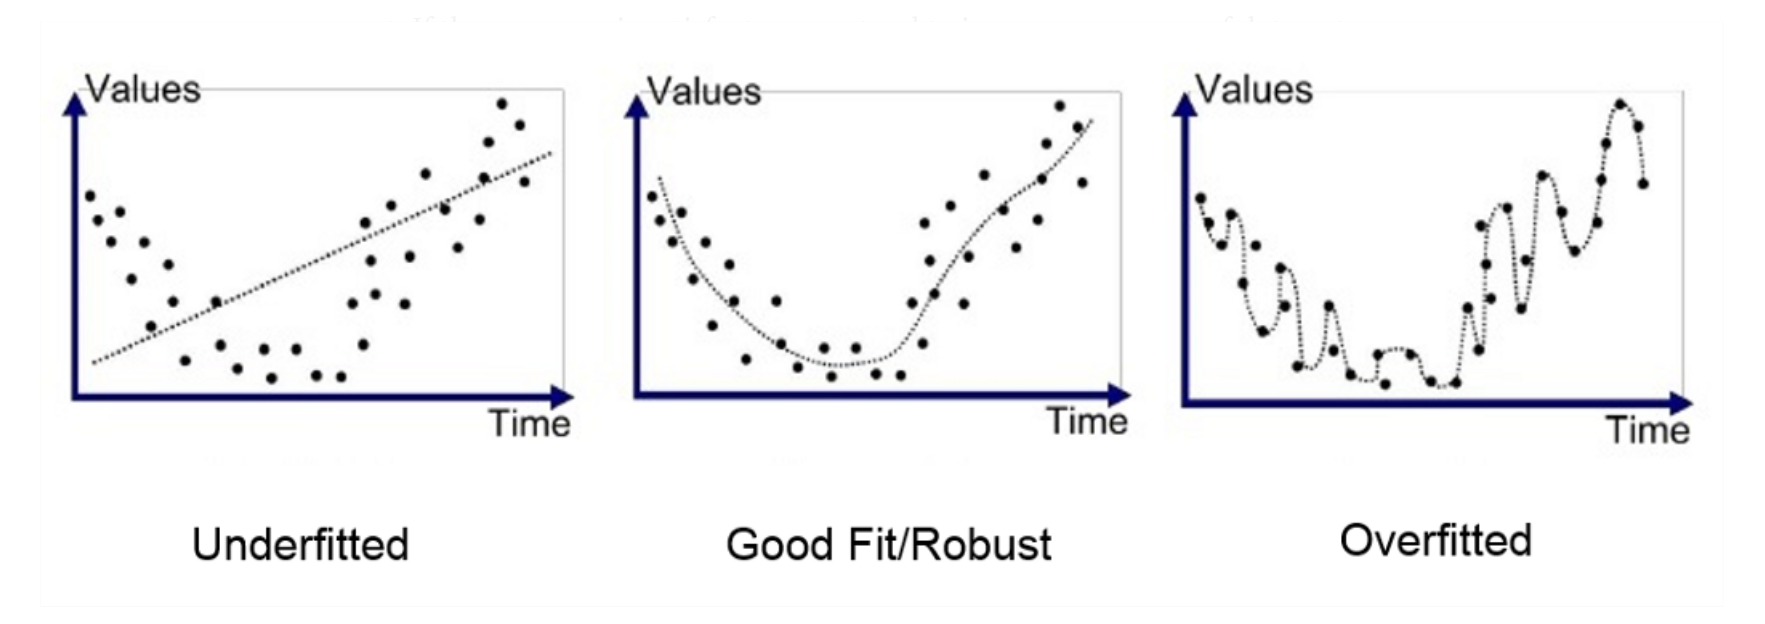
\includegraphics[width=0.7\textwidth]{figure/reg_lm_comparision.png}
% % \end{minipage}
% %  \normalsize
% % \begin{minipage}{0.4\textwidth}
% %   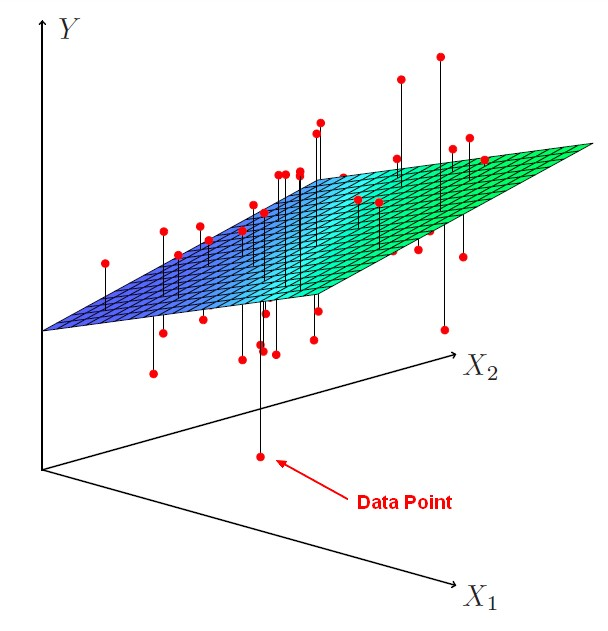
\includegraphics[width=0.7\textwidth]{figure/regression_hyperplane.jpg}
% % \end{minipage}
% 
% \end{frame}
% 
% % ------------------------------------------------------------------------------
% 
% \LARGE
% \begin{frame}{\textcolor{gray!80}{KNN} ~~ Functionality}
% \normalsize
% \vspace{-0.5cm}
% \noindent \textcolor{gray!80}{\rule{\textwidth}{1pt}}
% 
% \vspace{0.3cm}
% 
% \footnotesize
% 
% \textbf{\textcolor{gray!80}{Empirical risk}}
% 
% \begin{itemize}
% 
% \item XX
%   
%   
% \end{itemize}
% 
% 
% \medskip
% 
% \textbf{\textcolor{gray!80}{Optimization}} ~~
% XX
% 
% \medskip
% 
% \textbf{\textcolor{gray!80}{Hyperparameter}} XX
% 
% \end{frame}
% 
% % ------------------------------------------------------------------------------
% 
% 
% 
% 
% % \textbf{Advantages}
% % \begin{itemize}
% % \item simple adabtle to problem 
% % \item accuarate
% % \item easy to understand
% % \item few parameters to tune
% % \end{itemize}
% % 
% % 
% % \textbf{Disadvantages}
% % \begin{itemize}
% % \item memory intensive
% % \item computationally costly --> all training data might be involved in the decision making
% % \item slow performance
% % \item wrong distance measure can lead to inaccurate results 
% % \item k must be selected
% % \end{itemize}
% % \end{frame}
% 
% 
% 
% \LARGE
% \begin{frame}{\textcolor{gray!80}{KNN} ~~ Pro's \& Con's}
% \normalsize
% \vspace{-0.5cm}
% \noindent \textcolor{gray!80}{\rule{\textwidth}{1pt}}
% 
% \vspace{0.3cm}
% 
% \footnotesize
% 
% 
% \begin{columns}[onlytextwidth]
%   \begin{column}{0.5\textwidth}
%     \textbf{\textcolor{gray!80}{Advantages}}
%     \footnotesize
%     \begin{itemize}
%       \item[$\textbf{\textcolor{gray!80}{+}}$] XX
%     \end{itemize}
%   \end{column}
% 
%   \begin{column}{0.5\textwidth}
%     \textbf{\textcolor{gray!80}{Disadvantages}}
%     \footnotesize
%     \begin{itemize}
%       \item[$\textbf{\textcolor{gray!80}{-}}$] XX
%     \end{itemize}
%   \end{column}
% \end{columns}
% 
% \vfill
% 
% \small
% 
% \fbox{\parbox{\textwidth}{
% \centering
% \textbf{XX}}}
% 
% \end{frame}
% 
% % ------------------------------------------------------------------------------
% 
% \LARGE
% \begin{frame}{\textcolor{gray!80}{KNN} ~~ Practical hints}
% \normalsize
% \vspace{-0.5cm}
% \noindent \textcolor{gray!80}{\rule{\textwidth}{1pt}}
% 
% \vspace{0.3cm}
% 
% \footnotesize
% 
%   \textbf{\textcolor{gray!80}{Choice of regularization parameter  $\lambda$}} \\
%   \smallskip
%  XXXX
%  
%  
% 
% \lz
% 
%   \textbf{\textcolor{gray!80}{Implementation}} \\
%   \smallskip
%   R: package for regularized linear model \code{XXX}\\
%   Python: \code{XX} from package \code{XXX}, package for XXXX \code{statsmodels.api}
% 
% \end{frame}
% 
% % ------------------------------------------------------------------------------

\endlecture

\end{document}








